\section{Dokumentation der Implementierung}

% Sollte größter Teil werden
% - High level overview?
% - Wie läuft das auf meinem System?
% - Code Dokumentation / Entwicklerdokumentation




%%%%%%%%%%%%%%%%%%%%%%%%%%%%%%%%%%%%%%%%%%%%%%%%%%
% Abschnitt - Grober Überblick
%%%%%%%%%%%%%%%%%%%%%%%%%%%%%%%%%%%%%%%%%%%%%%%%%%


%%%%%%%%
% Highlevel
% ca 1-2 Seiten
% Buzzwords, grober Überriss
\subsection{Übersicht}

% TODO Ein bisschen mehr details
Das Problem fordert eine Unterteilung in drei wesentliche Bausteine, wie sie in \autoref{fig:architekturuebersicht} zu sehen sind.
Eine Benutzeroberfläche in einem Web Browser des Benutzers (“Frontend”), welches die Benutzerinteraktionen entgegennimmt und mit dem Backend kommuniziert.
Ein Backend-Host übernimmt dazu die Kommunikationsfunktion, verwaltet die eingehenden Rechenaufträge und verteilt sie an die Backend-Worker. Das Ergebnis dieser Berechnung sendet der Host dann an das Frontend zurück.
Die Backend-Worker nehmen die zugewiesenen Rechenaufträge entgegen und führen die eigentlichen Berechnungen verteilt aus.

\begin{figure}
	% Bindet das als PDF exportierte pptx ein -> vektorgrafik
	% -> pptx bearbeiten statt pdf
	\centering
	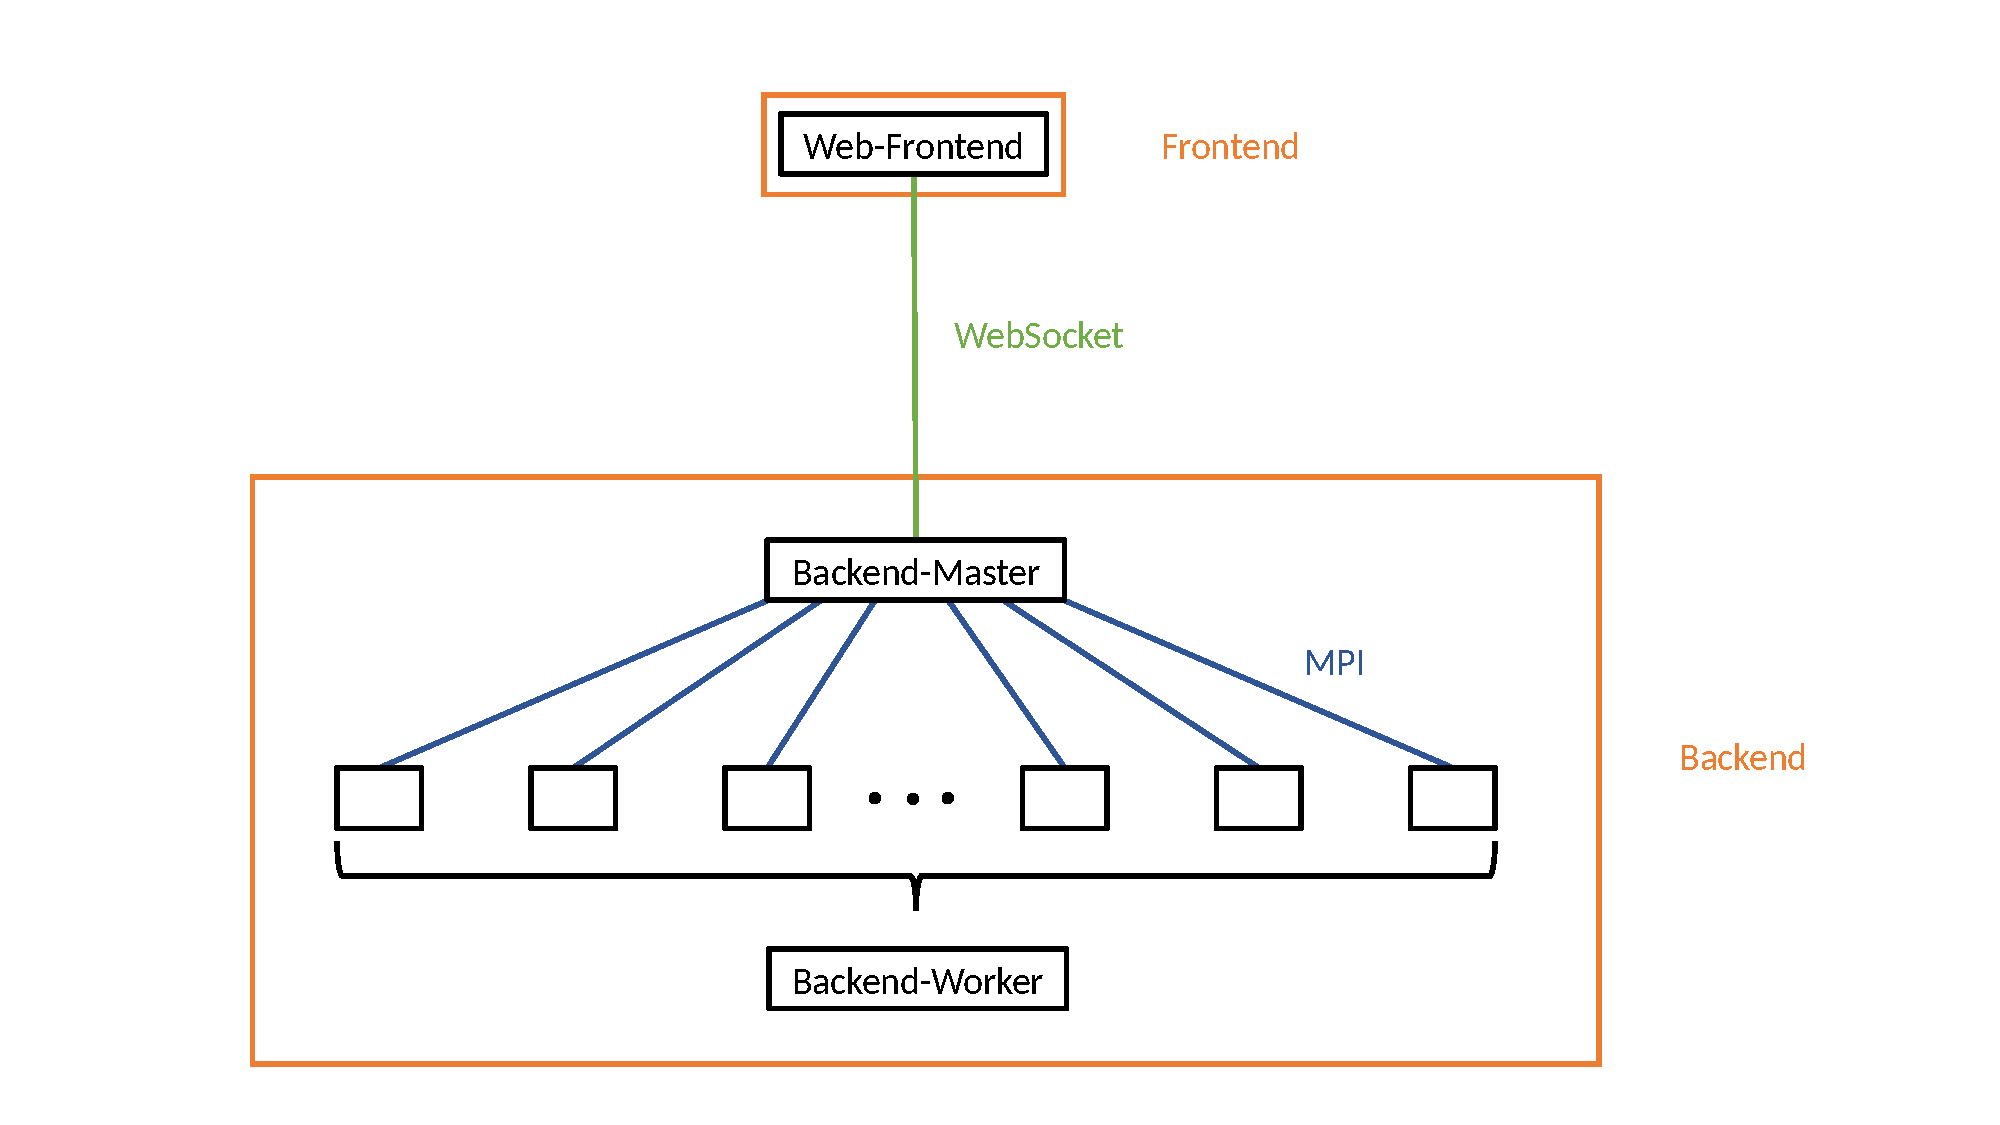
\includegraphics[width=0.98\linewidth]{img/Implementierung/Kommunikation.pdf}
	\caption{Architekturübersicht}
	\label{fig:architekturuebersicht}
\end{figure}

%%%%%%%%
% Middle level
% ca 2-3 Seiten
% Skripte, libraries/packages, Setup
% beispielbilder /output
% getestete Systeme (ARM/Raspi, Debian stretch, x86)
% mindeste was in README.md im master liegen sollte
% viel bereits in READMEs der zugehörigen Ordner zusammengefasst
% backend-deployment -> Niels
% frontend-deployment -> Max
\subsection{Installation der Anwendung}

Um das System zu installieren, muss das Repository mit \verb|git|\footnote{\url{https://git-scm.com/}} lokal geklont werden. Dabei werden die Quelldateien für
das Front- sowie Backend heruntergeladen.

\begin{figure}[h!]
	\begin{lstlisting}[language=bash, caption={Klonen des Repositorys}]
git clone https://gitlab.lrz.de/lrr-tum/students/eragp-mandelbrot.git
        \end{lstlisting}
\end{figure}

\subsubsection{Lokales Backend}
Eine lokale Installation des Backends zu Entwicklungszwecken ist durch einen Docker\footnote{\url{https://www.docker.com/}} Container möglich.
Dieser bietet eine ähnliche Umgebung zu der des Clusters und ermöglicht schnellere Feedbackzyklen.

\begin{figure}[h!]
	\begin{lstlisting}[language=bash, caption={Starten der Entwicklungsumbegung des Backends}]
# Systemabhängige Installation der Docker Anwendung
$ sudo apt install docker
cd backend/ && ./run_docker.sh
Starting the Build Process
...
Host: Core 37 ready!
# ^C beendet das Backend und verbindet sich mit der shell des Containers
^C[mpiexec@9cc2d5ac2cd1] Sending Ctrl-C to processes as requested
[mpiexec@9cc2d5ac2cd1] Press Ctrl-C again to force abort
# exit schliesst die shell des Containers
root@9cc2d5ac2cd1:~/eragp-mandelbrot/backend# exit
        \end{lstlisting}
\end{figure}

Das \verb|run_docker.sh| Skript lädt das benötigte Basis Image, welches alle benötigen Bibliotheken bereits enthält, herunter und erstellt basierend darauf
den Entwicklungscontainer. In diesen werden dann die Aktuellen Quelldateien hinein kopiert und kompiliert, wonach das Backend mit Adresse
\verb|ws://localhost:9002| gestartet wird.

\subsubsection{Backend auf HimMUC Cluster}

\begin{quotation}
	[Der] HimMUC ist ein flexibler Cluster von ARM-Geräten, bestehend aus 40 Raspberry Pi 3 sowie 40 ODroid C2 Single-Board-Computers (SBC).\footnote{\url{http://www.caps.in.tum.de/himmuc/}}
\end{quotation}

\paragraph{Schnellstart}

Um das Programm auf dem HimMUC Cluster zu starten, wurde ein
Python Skript erstellt, das alle notwendigen Schritte übernimmt.
Es führt die Befehle aus \autoref{par:detailed_himmuc} aus, es kann daher bei Problemen zur Fehlerbehebung herangezogen werden.

Stellen sie zunächst sicher, dass sie ein Konto mit Zugangsberechtigungen auf dem HimMUC Cluster besitzen.
Um den eigenen Quellcode auf dem Cluster zu kompilieren muss für die korrekte Funktionsweise des Skriptes zudem
ihr SSH-Key auf dem Cluster abgelegt sein\footnote{siehe \href{https://www.ssh.com/ssh/copy-id}{\texttt{ssh-copy-id}}}.

Außerdem sollten folgende Programme lokal installiert sein:
\begin{itemize}
	\item \verb|rsync|
	\item \verb|ssh|
	\item \verb|python3| (3.5 oder neuer)
\end{itemize}

Starten sie anschließend aus dem Ordner \verb|backend/| den Befehl aus \autoref{shell:start_himmuc}

\begin{figure}[h!]
	\begin{lstlisting}[language=bash, caption={Start der Entwicklungsumbegung auf dem HimMUC}, label={shell:start_himmuc}]
python3 himmuc/start_himmuc.py <Rechnerkennung> <Anzahl Prozesse> <Anzahl Rechenknoten> 
    \end{lstlisting}
\end{figure}

Das Ergebnis wird ähnlich zu \autoref{shell:start_himmuc_example} aussehen.
Details zu weiteren Optionen des Skripts sind via \verb|--help| verfügbar.

\begin{figure}
	\begin{lstlisting}[language=bash, caption={Beispielausgabe bei Start der Entwicklungsumbegung auf dem HimMUC}, label={shell:start_himmuc_example}]
$ eragp-mandelbrot/backend$ python3 himmuc/start_himmuc.py muendler 10 9
Uploading backend...  sending incremental file list
backend/himmuc/start_backend.py
          3,897 100%    3.05MB/s    0:00:00 (xfr#1, to-chk=35/62)
done
Start mandelbrot with 1 host and 9 workers on 9 nodes... started mandelbrot
Search host node... srun: error: Could not find executable worker
odr00 found
Establish port 9002 forwarding to host node odr00:9002 ... established
System running. Websocket connection to backend is now available at
        ws://himmuc.caps.in.tum.de:9002
Press enter (in doubt, twice) to stop Warning: Permanently added the ED25519 host key for IP address '10.42.0.54' to the list of known hosts.
# Enter

Stopping port forwarding... stopped (-9)
Stopping mandelbrot host and workers... stopped (-9)
    \end{lstlisting}
\end{figure}

\paragraph{Detaillierter Start}\label{par:detailed_himmuc}

Um Mandelbrot manuell auf dem Host-System zu installieren,
müssen zunächst die notwendigen Bibliotheken installiert werden.
Eine Anleitung dazu findet sich in \autoref{par:himmuc_install_libs}.
Dies muss nur einmal ausgeführt werden, anschließend können die
Programme wie in \autoref{par:himmuc_build_backend} beschrieben kompiliert werden.
Ist dies nicht gewünscht oder erledigt muss das Backend lediglich noch wie
in \autoref{par:himmuc_run_backend} beschrieben gestartet werden.


\paragraph{Lokale Installation der Bibliotheken}\label{par:himmuc_install_libs}


Da hierbei davon ausgegangen wird, dass keine root-Rechte auf dem
Server existieren, werden die Bibliotheken hier lokal in \verb|~/.eragp-mandelbrot|
installiert.
Achten Sie darauf, dass sie Schreibrechte auf dem Ordner haben und
falls sie einen anderen Ordner verwenden wollen,
ersetzen sie jedes Vorkommen des Pfades durch ihren Pfad (insbesondere in der Datei \verb|CMakeLists.txt|).
Die MPI-Bibliothek ist auf dem HimMUC Cluster bereits vorinstalliert
und muss daher nicht mehr aufgesetzt werden.
\begin{figure}[h!]
	\begin{lstlisting}[language=bash, caption={Erstellen des Installationsordners}]
mkdir ~/.eragp-mandelbrot
    \end{lstlisting}
\end{figure}

Die 'Header-only' Libraries \verb|websocketpp| und \verb|rapidjson| müssen
lediglich an einen fixen Ort kopiert werden.
Dies erledigen die Befehle aus \autoref{shell:install_header_libs}.

\begin{figure}[h!]
	\begin{lstlisting}[language=bash, caption={Lokale Installation der Bibliotheken \texttt{websocketpp} und \texttt{rapidjson}.}, label={shell:install_header_libs}]
mkdir "~/.eragp-mandelbrot/install"
cd "~/.eragp-mandelbrot/install"
# Installation von websocketpp
git clone --branch 0.7.0 https://github.com/zaphoyd/websocketpp.git websocketpp --depth 1
# Installation von rapidjson
git clone https://github.com/Tencent/rapidjson/
    \end{lstlisting}
\end{figure}


Aus der Bibliothek \verb|boost| muss die Teilbibliothek \verb|boost_system| lokal kompiliert werden
Dazu werden die Befehle aus \autoref{shell:install_boost} ausgeführt,
um die Version 1.67.0 herunterzuladen, zu entpacken und lokal zu installieren.
Beachten Sie, dass das kompilieren auch wie in \autoref{par:himmuc_build_backend} beschrieben
von einem der Boards ausgeführt werden muss.

\begin{figure}[h!]
    \begin{lstlisting}[language=bash, caption={Lokale Installation der Bibliothek boost.}, label={shell:install_boost}]
# Erstellen der notwendigen Ordnerstrukturen
mkdir "~/.eragp-mandelbrot/install"
mkdir "~/.eragp-mandelbrot/local"
# Einrichten des Internetproxys
export http_proxy=proxy.in.tum.de:8080
export https_proxy=proxy.in.tum.de:8080
# Herunterladen und kompilieren der Boost-Bibliothek
cd "~/.eragp-mandelbrot/install"
wget "https://dl.bintray.com/boostorg/release/1.67.0/source/boost_1_67_0.tar.bz2"
tar --bzip2 -xf boost_1_67_0.tar.bz2
cd boost_1_67_0
./bootstrap.sh --prefix="$HOME/.eragp-mandelbrot/local/" --with-libraries=system
./b2 install
    \end{lstlisting}
\end{figure}

\paragraph{Kompilieren des Backends}\label{par:himmuc_build_backend}

Stellen Sie zunächst sicher, dass auf dem Cluster die Quelldateien des Backendes (im Ordner \verb|backend/|) liegen
(zum Beispiel über \verb|rsync| oder indem sie das Repository dort auch klonen)
Zum Kompilieren des Backends sollte sich auf einen Raspberry Pi oder ODroid
per ssh eingeloggt werden\footnote{Es existiert ein Entwicklerzugang zu einem geteilten Raspberry Pi über die Adresse \url{sshgate-gepasp.in.tum.de}. Dieser wird auch vom Pythonskript genutzt}

Auf dem Board, aus dem Ordner des Backendquellcodes müssen Sie zum kompilieren
des Backendes die Befehle aus \autoref{shell:himmuc_compile_backend} ausführen.

\begin{figure}[h!]
	\begin{lstlisting}[language=bash, caption={Kompilieren des Backends}, label={shell:himmuc_compile_backend}]
# Erstellen und betreten eines build Ordners
mkdir build
cd build
# Aktivieren der MPI Bibliothek
module load mpi
# Kompilieren
cmake ..
make
    \end{lstlisting}
\end{figure}


\paragraph{Ausführen des Backends}\label{par:himmuc_run_backend}

Um das Backend auf dem HimMUC Cluster laufen zu lassen, muss sich zunächst darauf per ssh eingeloggt werden.
Damit für das Frontend kein Unterschied dazwischen besteht, ob das Backend im Dockercontainer , oder
auf einem externen Server ausgeführt wird, ist bei der ssh-Verbindung der Port 9002
des \verb|himmuc.caps.in.tum.de|-Servers an den lokalen Port 9002 gebunden.
So ist das Backend stets unter \url{localhost:9002} verfügbar.
Der zugehörige Befehl zum Login lautet demnach:

\begin{lstlisting}[language=bash]
ssh <rechnerkennung>@himmuc.caps.in.tum.de -L localhost:9002:localhost:9002
\end{lstlisting}

Anschließend muss aus dem Ordner, in dem die ausführbaren Dateien liegen,
für gewöhnlich also der \verb|~/.eragp-mandelbrot/build/| Ordner,
folgender Befehl ausgeführt werden:

\begin{lstlisting}[language=bash]
srun -p <odr|rpi> -n <number of workers+1> -N <number of nodes/raspis> -l --multi-prog <path to eragp-mandelbrot/backend>/himmuc/run.conf &
ssh -L 0.0.0.0:9002:localhost:9002 -fN -M -S .tunnel.ssh <odr|rpi><host number>
\end{lstlisting}

Dabei bestimmt \verb|-n| die Anzahl der laufenden Prozesse (Also Hostprozess und Workerprozesse)
und \verb|-N| die Anzahl zu verwendender Rechenknoten.
Damit anschließend noch alle Anfragen an den Websocketserver auf dem Hostknoten weitergeleitet werden,
muss noch der Port 9002 des \url{himmuc.in.caps.tum.de}-Servers an den Port 9002 des Rechenknotens gebunden werden,
auf dem der Hostprozess läuft.
Der korrekte Knoten ist dabei der Ausgabe des \verb|srun|-Befehles zu entnehmen.
Eine beispielhafte Ausgabe ist in \autoref{shell:himmuc_running_backend_example} zu sehen.

\begin{figure}[h]
	\begin{lstlisting}[language=bash, caption={Beispielhafter Start des Backends. Hierbei ist der Knoten des Hostprozesses \texttt{rpi03}.}, label={shell:himmuc_running_backend_example}]
muendler@vmschulz8:~/eragp-mandelbrot/backend/build$ srun -N4 -n5 -l --multi-prog ../himmuc/run.conf
srun: error: Could not find executable worker
4: Worker: 4 of 5 on node rpi06
2: Worker: 2 of 5 on node rpi04
3: Worker: 3 of 5 on node rpi05
0: Host: 0 of 5 on node rpi03
0: Host init 5
1: Worker: 1 of 5 on node rpi03
0: Core 1 ready!
1: Worker 1 is ready to receive Data.
2: Worker 2 is ready to receive Data.
0: Listening for connections on to websocket server on 9002
0: Core 2 ready!
3: Worker 3 is ready to receive Data.
0: Core 3 ready!
4: Worker 4 is ready to receive Data.
0: Core 4 ready!
muendler@vmschulz8:~/eragp-mandelbrot/backend/build$ ssh ssh -L 0.0.0.0:9002:localhost:9002 -fN -M -S .tunnel.ssh rpi03
    \end{lstlisting}
\end{figure}

\paragraph{Stoppend des Backends}

Um das Backend wieder zu stoppen, müssen der ssh-Tunnel zur Verbindung der Ports
und der \verb|srun|-Prozess gestoppt werden.
Letzterer lässt sich nach dem dämonisieren im vorigen Aufruf nur über die Prozess-ID finden.
Diese zeigt das Tool \verb|ps| an.
\begin{lstlisting}[language=bash]
ssh -S .tunnel.ssh -O exit rpi<host number>
# To stop the node allocation
ps -eo comm,pid | grep srun
kill <srun pid>
\end{lstlisting}

\subsubsection{Installation des Frontends}
Das Frontend ist in TypeScript\footnote{\url{https://www.typescriptlang.org/}} (erweiterung von JavaScript\footnote{\url{https://en.wikipedia.org/wiki/JavaScript}})
geschrien und kann somit auf einem beliebigen Endgerät mit einem modernen Webbrowser ausgeführt werden.
Um eine Version lokal zu starten, muss die Paketverwaltung npm\footnote{\url{https://www.npmjs.com/}} installiert werden. Diese verwaltet alle
für das Frontend benötigten Bibliotheken und installiert diese lokal.

\begin{figure}[h!]
	\begin{lstlisting}[language=bash, caption={Starten des Frontends mit beispielhafter Ausgabe}]
# Systemabhängige Installation der npm Paketverwaltung
sudo apt install npm
# Installiert benötigte Bibliotheken und startet WebServer
cd frontend/ && npm install ; npm start
...
Version: webpack 4.25.1
Time: 7230ms
Built at: 12/28/2018 10:48:32 PM
        Asset      Size  Chunks             Chunk Names
   index.html  1.65 KiB          [emitted]
mandelbrot.js  11.7 MiB    main  [emitted]  main
    style.css   519 KiB    main  [emitted]  main
Entrypoint main = style.css mandelbrot.js
...
        \end{lstlisting}
\end{figure}

Das Kommando \verb|npm start| startet dabei einen lokalen WebServer, welcher eine kompilierte Version des Frontends
unter der Adresse \verb|http://localhost:3000| anbietet. Danach wird der Standardwebbrowser des Systems verwendet, um diese
URL zu öffnen.

%%%%%%%%
% Low level
% was muss ich als entwickler wissen
% tiles, parallelisierung, structs/klassen, struktur des projekts

% Zuordnung klasse -> Dokumentation
% backend
%   *.main.cpp, init -> Niels DONE
%   include Ordner und CMake -> Niels DONE
%   balancer + tests -> Florian
%   mandelbrot -> Florian (außer MandelbrotSIMD -> Niels DONE)
%   actors
%      Worker -> Tobi
%      Host
%         websocket-funktionen -> Niels
%         Rest -> Tobi
%           + Parallelisierungskonzept (+ welche MPI Method, warum)
%   structs/Netzwerk -> Tobi/Niels/Florian
%   dev-environment (was ist docker und wie/warum) -> Max
% frontend
%    connection -> Niels
%    tileDisplay -> Max
%        TileDisplay.ts
%            Prinzip 
%            genauer Ablauf/Funktionen
%               + Shader
%        WorkerLayer.ts
%           + Gruppierung
%        MatrixView.ts + RegionOfInterest.ts
%        Project.ts
%    visualization -> Niels
%    misc -> Max

\subsection{Erläuterung des Backends}

\subsection{Implementierung der Mandelbrotberechnung}

Zur hardwarenahe Berechnung der Mandelbrotmenge wird ein sogenanntes Backend gestartet.
Das in C++ programmierte Teilprojekt nimmt Rechenaufträge von einem Nutzer durch ein Frontend entgegen (auch
ein solches wird bereitgestellt), zerlegt sie und verteilt sie per MPI auf dedizierte Rechenknoten.
Dazu besteht das Backend aus zwei ausführbaren Dateien, \verb|host| und \verb|worker|.

\subsubsection{Inkludierte Header und CMake Anweisungen}

Die zusammenstellung der ausführbaren Dateien wird in CMake definiert.
Dabei unterscheiden sich diese lediglich in den eingebundenen Quelldateien:
In die Datei \verb|host| werden \verb|host.main.cpp| und \verb|actors/Host.cpp| eingebunden, während
in \verb|worker| \verb|worker.main.cpp| und \verb|actors/Worker.cpp| eingebunden werden.

Diese und alle weiteren Build-Vorgaben werden in der Datei \verb|CMakeLists.txt| für
\verb|cmake|\footnote{Ein Programm, welches die Erstellung von Makefiles vereinfacht in dem es sie automatisch an die Umgebung des Build-Systems anpasst. \url{https://cmake.org/}}
in der hier beschriebenen Reihenfolge spezifiziert.
Es sollte hierbei eine CMake-Version über 3.7.0 gewählt werden und die C++11 Standards\footnote{\url{https://isocpp.org/wiki/faq/cpp11}} werden vorrausgesetzt.
Zudem werden für das Projekt "Mandelbrot" werden alle Dateien im Order \verb|include| eingebunden.
In diesem Ordner liegen die Header-Dateien für alle projektinternen C++-Quelldateien.
Anschließend werden alle C++-Quelldateien (Endung "\verb|.cpp|") aus dem Ordner \verb|src| in einer Liste gesammelt, mit Ausnahme jedoch der oben genannten, exklusiven Quelldateien.
Die erzeugte Liste und die jeweils exklusiven Dateien werden dann den ausführbaren Dateien \verb|host| und \verb|worker| zugeordnet.

Um die verwendeten Bibliotheken verfügbar zu machen werden anschließend die Header der installierten MPI-Bibliothek
sowie die Header der Bibliotheken rapidjson\footnote{\url{http://rapidjson.org}}, websocketpp\footnote{\url{https://github.com/zaphoyd/websocketpp}} und boost\footnote{\url{https://www.boost.org/}}
Diese werden respektive verwendet um JSON zu parsen und enkodieren, Websocket-Verbindungen aufzubauen und darüber zu kommunizieren sowie um diese Bibliothek zu unterstützen.
Da für die boost Bibliothek dabei Header nicht genügen und die systemweite Verfügbarkeit der kompilierten boost-Bibliothek nicht garantiert werden kann, wird die Teilbibliothek boost\_system statisch
in die ausführbaren Datei \verb|host| eingebunden.

Zuletzt werden über Compilerflags alle Kompilierfehler und -warnungen aktiviert sowie die POSIX-Thread-Bibliothek eingebunden
und spezielle Flags für die Websocketlibrary und MPI gesetzt.

\subsubsection{Mainfunktion und Initialisierung}

Zur Initialisierung der Prozesse muss zunächst die MPI-Umgebung aktiviert und abgerufen werden.
Dies geschieht für beide Programme gleich, über die Initialisierungsfunktion in \autoref{src:init.cpp}.
Sie erwartet lediglich eine Beschreibung des Prozesses für den Log und eine Initialisierungsfunktion,
die erst zurückkehrt, wenn das Programm abgeschlossen ist und MPI beendet werden soll.
Die Funktion muss als Parameter den Rang bzw. die Id des aktuellen MPI-Prozesses und die Anzahl der initialisierten
Prozesse entgegen nehmen.

Ein beispielhafter Aufruf ist in \autoref{src:host.main.cpp} zu sehen. Damit wird MPI initialisiert und nach der
erfolgreichen Initialisierung der eigentliche \hyperref[cls:Host]{Host-Prozess} über \verb|Host::init| gestartet.

\begin{figure}[h]
	\lstinputlisting[caption={Initialisierung des Host-Prozesses in host.main.cpp}, label={src:host.main.cpp}]{../../backend/src/host.main.cpp}
\end{figure}

\begin{figure}
	\lstinputlisting[caption={Initialisierung der MPI-Prozesse in init.cpp}, label={src:init.cpp}, firstline=15, lastline=39, firstnumber=15]{../../backend/src/init.cpp}
\end{figure}

\subsection{Host Funktionalitäten}\label{cls:Host}

\subsubsection{Websocketverbindung}

Direkt nach der Initialisierung des Host-Programms in \autoref{src:Host.cpp::init.websocket}, wird ein separater Thread gestartet, der über Websocket
Anfragen zur Berechnung einer Region entgegennimmt sowie ein Thread, der berechnete Regionen an den verbundenen Client übergibt.
Die Methode \verb|Host::start_server| initialisiert dabei lediglich den Websocketserver mit den Methoden zum Behandeln geöffneter und geschlossener Verbindungen und
einer Methode um Nachrichten des Clients zu behandeln, \hyperref[cls:Host::handle_region_request]{\texttt{Host::handle\_region\_request}}.
Der zweite gestartete Thread führt die Methode \hyperref[cls:Host::send]{\texttt{Host::send}} aus.
Zudem wird der Websocketserver mit \verb|server.init_asio()| mit der Transport Policy "transport::asio"
konfiguriert, sodass Multithreadzugriff auf Sende- und Empfangsmethoden problemlos möglich ist \cite{websocketppManual}.

\begin{figure}
	\lstinputlisting[caption={Starten des Websocketservers bei der Initialisierung des Host-Programmes in Host.cpp}, label={src:Host.cpp::init.websocket}, firstline=382, lastline=393, firstnumber=382]{../../backend/src/actors/Host.cpp}
\end{figure}

\paragraph{Host::handle\_region\_request}\label{cls:Host::handle_region_request}

Die Methode versucht, den Inhalt der empfangenen Nachricht als JSON zu dekodieren und entnimmt die für das struct Region
notwendigen Werte unter gleichem Namen dem Objekt, das unter dem Schlüssel \verb|"region"| in der geparsten Anfrage gespeichert ist.
Außerdem erwartet es unter dem Schlüssel \verb|"balancer"| einen String, der den zu wählenden Lastbalancierer bestimmt und unter dem Schlüssel \verb|"type"| den String \verb|"regionRequest"|.
Mögliche Zeichenketten hierfür sind in den Klassen der Balancierer unter \verb|backend/src/balancer| in der globalen Variable
\verb|Klassenname::NAME| gespeichert.
Ein Beispiel für einen Namen kann in \autoref{src:PredictionBalancer.NAME} gefunden werden:

\begin{figure}[h]
	\lstinputlisting[caption={Namensdefinition des PredictionBalancers}, label={src:PredictionBalancer.NAME}, firstline=11, firstnumber=11, lastline=11]{../../backend/src/balancer/PredictionBalancer.cpp}
\end{figure}

Ein Beispiel für eine gültige Regionsanfrage ist in \autoref{src:regionRequest.json} zu finden.
Einerseits wird hierbei eine Region in komplexen Koordinaten beschrieben, wobei der obere linke Punkt $(maxImag, minReal)$
und der rechte untere Punkt $(minImag, maxReal)$ in der komplexen Ebene einen zu berechnenden Bereich aufspannen.
Da die reelle Ebene jedoch beliebig genau aufgelöst werden kann, muss zudem noch die Anzahl an Pixeln
pro Seite des Rechteckes definiert werden, \verb|width| und \verb|height|.
Wie in \autoref{fig:concept_coordinates} zu sehen, ist zudem der horizontale Offset und vertikale Offset
die linke obere Koordinate der Region bezüglich der gesamten sichtbaren Anfrage in Pixeln (diese Werte
gewinnen in den Regionsaufteilungen an Bedeutung).
Der Wert \verb|validation| ist technisch gesehen nicht mehr notwendig, wird aber mit dem Zoom-wert der Leafletkarte gefüllt
um zu vermeiden dass Regionsdaten von zuvor berechneten Regionen falsch verwendet werden.

\begin{figure}
	\lstinputlisting[caption={Eine gültige Anfrage einer Region in JSON}, label={src:regionRequest.json}, language=json]{./code/regionRequest.json}
\end{figure}

\begin{figure}
    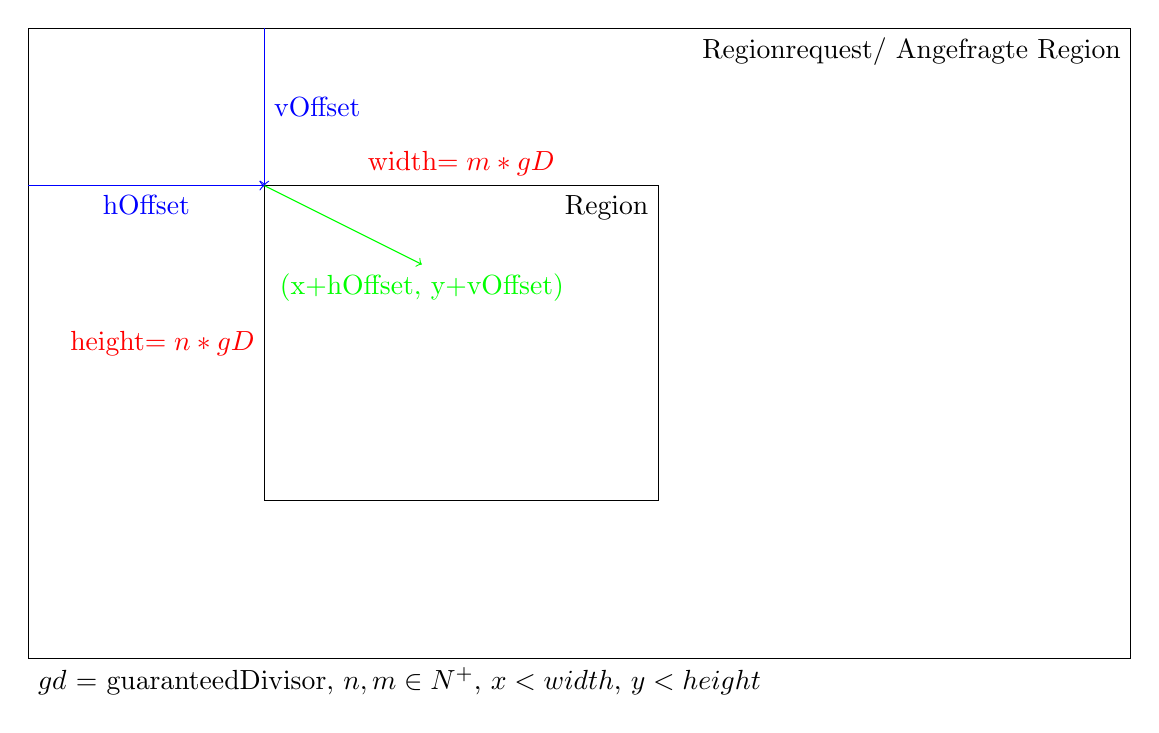
\begin{tikzpicture}
        % Superregion
        \draw (0,0) rectangle (14,8) node[below left] {Regionrequest/ Angefragte Region};
        % subregion
        \draw (3,2) rectangle (8,6) node[below left] {Region};
        % width height
        \draw (3,6) -- node[above, red] {width$=m*gD$} (8,6);
        \draw (3,6) -- node[left, red] {height$=n*gD$} (3,2);
        % vOffset/hOffset
        \draw[blue, ->] (3,8) -- (3,6) node[midway, anchor=west] {vOffset};
        \draw[blue, ->] (0,6) -- (3,6) node[midway, anchor=north] {hOffset};
        % x/y
        \draw[green, ->] (3,6) -- (5,5) node[below] {(x+hOffset, y+vOffset)};
        \draw (0, 0) node[below right] {$gd$ = guaranteedDivisor, $n,m \in \mathbb{N}^{+}$, $x < width$, $y < height$};
    \end{tikzpicture}
    \caption{Konzept der Kooridinaten in den Regionsobjekten. Alle Koordinaten beziehen sich auf die Darstellungsebene und sind daher in Pixeln.}
    \label{fig:concept_coordinates}
\end{figure}


Nach dem Parsen der Nachricht wird die Region global festgelegt und beim korrekten Lastbalancierer eine Zerlegung der angefragten Region über \verb|Balancer::balanceLoad| gestartet.

Jeder Region wird ein Worker zugewiesen.
Dabei ist der Rang des Workers, der eine Region berechnen soll genau der Index der Region in dem zurückgegebenen Array.
Ist ein Worker nicht verfügbar, so werden sein und alle folgenden Ränge um eins erhöht (siehe \autoref{src:Host.cpp.handle_region_request}).
Damit kann der Websocketprozess unabhängig von der tatsächlichen Verteilung den Rang des berechnenden Worker-Prozesses
bestimmen und in der Antwort an den Client zu der Aufteilung der Prozesse einfügen.
Die Struktur und eine gültige Antwort des Websocketservers kann \autoref{src:region.json} entnommen werden.

Nachdem die Aufteilung als Antwort auf die Anfrage dem Websocketprozess bereitgestellt wurde, werden die Teilregionen in eine per Mutexlock-gesicherte Datenstruktur
gelegt. Der MPI verwendende Thread, der diese Regionen anschließend an die Worker sendet wird über das Setzen des booleschen Wertes \verb|mpi_set_regions|
auf \verb|true| darüber informiert, dass neue Regionen zum versenden zur Verfügung stehen.

Indem die Regionaufteilung zuerst an das Frontend und anschließend an die Worker gesendet wird,
wird sichergestellt, dass das Frontend alle empfangenen Regionsdaten korrekt der angefragten Region zuordnen kann.
Dabei wird zwar Rechenzeit verschenkt, jedoch steigt durch die Erstellung sehr kleiner oder leerer Teilregionen
die Wahrscheinlichkeit, dass ein Arbeiter mit seiner Region zu früh abgeschlossen ist.
Würde dann dessen Region vor der Gesamtaufteilung beim Frontend ankommen, besteht die Gefahr,
dass es die Daten verwirft.

\begin{figure}
	\lstinputlisting[caption={Algorithmus zur Zuordnung von Regionen auf Worker in Host.cpp}, label={src:Host.cpp.handle_region_request}, firstline=231, firstnumber=231, lastline=240]{../../backend/src/actors/Host.cpp}
\end{figure}

\begin{figure}
	\lstinputlisting[caption={Ausschnitt aus einer gültigen Antwort auf die Region aus \autoref{src:regionRequest.json} in JSON}, label={src:region.json}, language=json]{./code/region.json}
\end{figure}

\paragraph{Host::send}\label{cls:Host::send}

Während ein Thread das Empfangen von Nachrichten übernimmt, behandelt diese Methode von den Workern fertig berechnete Regionen.
Er versendet in einer Dauerschleife Regionsdaten an den aktuell verbundenen Client.
Nach jedem Durchlauf oder wenn der Thread per \verb|notify| (oder auch durch mögliche andere Nebeneffekte) aufgeweckt wird,
überprüft er auf das Vorhandensein neuer Regionen, wählt die erste aus und entfernt sie aus der Datenstruktur.
Nachdem das Lock auf die geteilte Datenstruktur gelöst wurde, werden die Regionsdaten JSON codiert versendet.
Ein Beispiel für versendete Regionsdaten kann \autoref{src:regionData.json} entnommen werden.
Dabei wird der Punkt (x, y) in der gesendeten Region (Punkt (x+hOffset, y+vOffset) in der angefragten Region)
im Datenarray an Index $i = x + y * width$ gespeichert.
Ist keine Region in der Datenstruktur abgelegt wird per \verb|wait| auf eine Änderung gewartet.
Mithilfe der \verb|condition_variable|\footnote{\url{https://en.cppreference.com/w/cpp/thread/condition_variable}} \verb|Host::mpi_to_websocket_result_available|
nutzt sie die C++11 nativen mutex-Mechanismen um über das Vorhandensein neuer Regionen informiert zu werden.

\begin{figure}
	\lstinputlisting[caption={Ausschnitt aus den Daten einer versendeten Teilregion. Punkt (x,y) liegt in \texttt{"data"} an Index $i=x+y*width$.}, label={src:regionData.json}, language=json]{./code/regionData.short.json}
\end{figure}

\subsection{Lastbalancierung}\label{sec:load_balancing}
Um die Mandelbrotmenge effizient parallel zu berechnen, muss die Last gleichmäßig auf die Worker verteilt werden.
Die Aufgabe der Lastbalancierung besteht darin zu einer gegebenen Region und einer Anzahl von Workern eine solche Unterteilung in sogenannte Teilregionen zu finden.
Wichtig dabei ist, dass der garantierte Teiler von Höhe und Breite der Teilregionen dem der angeforderten Region entspricht.
Eine Tile (ein Bereich mit Breite und Höhe gleich dem garantierte Teiler\footnote{Eine Region lässt sich also immer in eine ganzzahlige Anzahl von Tiles aufteilen, vgl. \autoref{fig:leafletTiles}}, die Bezeichnung \textit{Tile} kommt aus dem Frontend) muss also als atomare Einheit betrachtet werden, da es sonst im Frontend zu Schwierigkeiten bei der Darstellung kommt.
Die Klassenstruktur der Lastbalancierer entspricht dem Strategy-Pattern\footnote{\url{https://sourcemaking.com/design_patterns/strategy}}. So kann der Balancierer zur Laufzeit leicht gewechselt werden und auch die Erweiterung des Projekts um eine weitere Strategie gestaltet sich einfach.
Was dabei genau beachtet werden muss findet sich im Teil \hyperref[lastbalancierung_erweiterung]{Erweiterung}.


Damit die Unterschiede zwischen guter und schlechter Lastverteilung deutlich werden, wurden hier verschiedene Strategien zur Lastbalancierung implementiert.

\subsubsection{Naive Strategie}

Bei der naiven Strategie (zu finden in den Klassen \verb|NaiveBalancer| und \\ \verb|RecursiveNaiveBalancer|) wird versucht den einzelnen Workern etwa gleich große Teilregionen zuzuweisen.
Dies geschieht allerdings ohne Beachtung der eventuell unterschiedlichen Rechenzeiten innerhalb der Teilregionen.
Die naive Strategie wurde hier in einer nicht-rekursiven und einer rekursiven Variante implementiert.

\paragraph*{Nicht-rekursive Variante}\label{lastbalancierung_naiv}
%non-recursive naive
Zur nicht-rekursiven Aufteilung wird zuerst die Anzahl der zu erstellenden Spalten und Zeilen berechnet.
Dazu wird der größte Teiler der Anzahl der Worker bestimmt. Dieser gibt die Anzahl der Spalten an, das Ergebnis der Division ist die Anzahl der Zeilen.
Damit ist sichergestellt, dass die Region in die richtige Menge von Teilregionen unterteilt wird.

Als nächstes wird die Breite und Höhe der Teilregionen berechnet. Hierbei ist wichtig, dass der garantierte Teiler erhalten wird.
Die Breite berechnet sich also durch:
\begin{equation*}
	\frac{region.width}{region.guaranteedDivisor * nodeCount} * region.guaranteedDivisor
\end{equation*}
Dabei ist \verb|nodeCount| die Anzahl der Worker und \verb|region| die zu unterteilende Region.
Es ist zu beachten, dass es sich hier um eine Ganzzahldivision handelt, deren Rest angibt, wie viele Teilregionen um \verb|region.guaranteedDivisor| breiter sind.
Die Höhe berechnet sich analog.

Bevor die eigentliche Aufteilung beginnt werden noch die Deltas für Real- und Imaginärteil bestimmt.
Diese geben an, wie breit bzw. hoch der Bereich der komplexen Ebene ist, den ein Pixel der Region überdeckt.
Die Deltas können über Methoden der Klasse Fractal berechnet werden.

Zur Aufteilung wird nun mittels zweier verschachtelter Schleifen über die Zeilen und Spalten iteriert.
Die benötigten Start- und Endpunkt der Teilregionen (also die linke obere Ecke und die rechte untere Ecke auf der komplexen Ebene) können nun mithilfe der Schleifenzähler und der Deltas bestimmt werden.
Zusätzlich wird noch der vertikale und horizontale Offset der Teilregion vom Startpunkt der Eingaberegion abgespeichert. Diese Information ermöglicht es die Region im Frontend einfach anzuzeigen.

Falls die aktuell betrachtete Teilregionen zu den Breiteren und/oder Höheren (s.o.) gehört, müssen alle Werte entsprechend angepasst werden.
Die letzte Teilregion einer Spalte bzw. Zeile wird immer so gewählt, dass sie auf jeden Fall mit dem Rand der Eingaberegion abschließt.

Die Teilregionen werden in einem Ergebnisarray gespeichert, welches dann zurückgegeben wird.

\paragraph*{Rekursive Variante}\label{lastbalancierung_naiv_rekursion}
% recursiveNaive
Die Grundidee der rekursiven Balancierung ist, die Region solange zu halbieren, bis man genug Teile für jeden Worker hat.
Dies funktioniert sehr gut, wenn die Anzahl der Worker eine 2er-Potenz ist.
Wenn das nicht der Fall ist, so müssen für einige Worker die Regionen öfters geteilt werden als für andere.
Die Anzahl der Blätter des Rekursionsbaumes (hier ein Binärbaum) muss also der Anzahl der Worker entsprechen.

Um die Werte, die während der rekursiven Auswertung benötigt werden, einfach weiterreichen zu können wurde die Struktur \verb|BalancingContext| definiert.
Diese beinhaltet einen Zeiger auf das Ergebnisarray (\verb|result|) und den aktuellen Index (\verb|resultIndex|) in dieses.
Zusätzlich ist in \verb|partsLeft| gespeichert, wie viele Teilregionen der jeweilige Rekursionsschritt noch erzeugen muss.
Auch die Deltas für Real- und Imaginärteil sind in der Struktur abgelegt, um wiederholte Berechnungen zu vermeiden.

Aus \verb|partsLeft| kann auch die Abbruchbedingung der Rekursion gefolgert werden:
\begin{equation}\label{lastbalancierung_rekursion_abbruch}
	partsLeft = 1
\end{equation}

Ist die Abbruchbedingung (\ref{lastbalancierung_rekursion_abbruch}) erfüllt, so genügt es die übergebene Region in das Ergebnisarray einzutragen und \verb|resultIndex| zu inkrementieren.
Ansonsten muss die Region halbiert werden. Ist die Region vertikal oder horizontal nicht mehr teilbar (d.h. \verb|region.width| bzw. \verb|region.height| $\leq$ \verb|region.guaranteedDivisor|), so wird in die andere Richtung geteilt.
Kann die Region in beide Richtungen geteilt werden, so wird parallel zur kürzeren Seite geteilt.
Dies gibt dem Lastbalancierer mehr Möglichkeiten die Trennlinie zwischen den Teilregionen zu setzen, was zu einer genaueren Teilung führt.
Wenn die Region unteilbar ist, so muss eine leere Region erzeugt werden.

Die beiden Hälften berechnen sich wie bei der Aufteilung auf zwei Worker mit der \hyperref[lastbalancierung_naiv]{nicht-rekursiven Strategie}.
Dann wird die Funktion für jede Hälfte rekursiv aufgerufen, wobei \verb|partsLeft| entsprechend halbiert wird.

\subsubsection{Strategie mit Vorhersage}

Bei dieser Strategie (zu finden in den Klassen \verb|PredictionBalancer| und \\ \verb|RecursivePredictionBalancer|) basiert die Aufteilung der Region auf einer Vorhersage über die Rechenzeit.
Die Teilregionen werden so gewählt, dass sie, entsprechend der Vorhersage, etwa einen ähnlichen Rechenaufwand haben.

\paragraph*{Bestimmung der Vorhersage}
% predicter
Die Vorhersage (\verb|struct Prediction|) wird von der Klasse Predicter angestellt.
Dazu wird die Region in einer sehr viel geringeren Auflösung berechnet.
Die benötigte Anzahl an Iterationen wird jeweils pro Tile abgespeichert.
So wird sichergestellt, dass der garantierte Teiler auch nach der Aufteilung noch gilt, da die Balancierer die Vorhersage Eintrag für Eintrag verarbeiten.
Die Genauigkeit der Vorhersage kann über das Attribut \verb|predictionAccuracy| gesteuert werden:
\begin{itemize}
	\item $predictionAccuracy > 0$: $(predictionAccuracy)^2$ Pixel werden pro Tile berechnet. Die Summe der Iterationen für die einzelnen Pixel ergibt die Vorhersage für die Tile.
	\item $predictionAccuracy < 0$: Für $(predictionAccuracy)^2$ Tiles wird ein Pixel in der Vorhersage berechnet. Es erhalten also mehrere Tiles diesselbe Vorhersage.
	\item $predictionAccuracy = 0$: Unzulässig, es wird ein Null-Pointer zurückgegeben.
\end{itemize}
Es ist wichtig eine gute Balance zwischen Güte und Geschwindigkeit der Vorhersage zu finden.
Zusätzlich beinhaltet die Vorhersage die Summen der benötigten Iterationen pro Spalte und Zeile, sowie die Gesamtsumme.
Auch die Deltas für Real- und Imaginärteil pro Tile und die Anzahl der Zeilen und Spalten werden angegeben.

Auch die Strategie mit Vorhersage wurde in einer rekursiven und in einer nicht-rekursiven Variante implementiert.

\paragraph*{Nicht-rekursive Variante}\label{lastbalancierung_vorhersage}
% non-recursive prediction
Für die nicht-rekursive Variante wird zuerst die benötigte Anzahl an Zeilen und Spalten bestimmt.
Dies geschieht genauso wie bei der naiven Strategie.

Die erzeugten Teilregionen sollen in etwa den gleichen Rechenaufwand haben. Dieser berechnet sich durch:
\begin{equation}\label{lastbalancierung_vorhersage_formel}
	desiredN = \frac{nSum}{nodeCount}
\end{equation}
Dabei ist \verb|nSum| die Gesamtsumme der Vorhersage und \verb|nodeCount| wieder die Anzahl der Worker.

Danach wird die Region erst in Spalten aufgeteilt und in einem zweiten Schritt wird dann die horizontale Unterteilung in Teilregionen vorgenommen.

Zur Aufteilung wird über die Spaltensummen in der Vorhersage iteriert (vgl. \autoref{src:PredictionBalancerAuszug.cpp}). Diese werden aufaddiert und bilden so den Zähler \verb|currentN|.
Sobald \verb|currentN| $\geq$ \verb|desiredN| gilt oder für alle restlichen Spalten nur noch je ein Eintrag in den Spaltensummen vorhanden ist, wird eine Spalte abgeschlossen.
Dazu werden \verb|maxReal| und \verb|width| aus den Zählern berechnet. Es ist wichtig \verb|maxReal| immer neu aus \verb|region.minReal| zu berechnen, anstatt nur das Delta aufzuaddieren, da sich sonst der Fehler, der bei Fließkommaaddition unvermeidbar ist, auch mit aufaddiert. \verb|minReal| und \verb|hOffset| stehen bereits in der Region \verb|tmp|, die Werte wurden bei der Berechnung der vorhergehenden Spalte bereits gesetzt.
Jetzt wird \verb|tmp| für die nächste Spalte vorbereitet, das heißt \verb|tmp.minReal| wird auf \verb|tmp.maxReal| gesetzt und \verb|tmp.hOffset| wird um \verb|tmp.width| erhöht. Ersteres vermeidet das Entstehen von Lücken zuverlässig.
Außerdem wird \verb|desiredN| für die verbleibenden Spalten nach (\ref{lastbalancierung_vorhersage_formel}) neu berechnet und die Zähler werden zurückgesetzt.
Bevor die Aufteilung der Spalte in Teilregionen startet, wird eine Kopie der Vorhersage erstellt, die nur die Werte für die aktuelle Spalte enthält.
Das Aufteilen einer Spalte in Teilregion geschieht analog zum Aufteilen in Spalten.

Die letzte Spalte wird gesondert behandelt: Sie muss so gewählt werden, dass sie den gesamten Rest der Eingaberegion abdeckt, ansonsten können Lücken entstehen.
Dies gilt genauso bei der Unterteilung der einzelnen Spalten.

\begin{figure}
	\lstinputlisting[caption={Aufteilung in Spalten (Auszug)}, label={src:PredictionBalancerAuszug.cpp}, firstline=23, lastline=70]{./code/PredictionBalancerAuszug.cpp}
\end{figure}

\paragraph*{Rekursive Variante}
% recursive prediction
Die rekursive Variante der Strategie mit Vorhersage verwendet dasselbe Rekursionsschema wie ihr \hyperref[lastbalancierung_naiv_rekursion]{naives Gegenstück}.
Die Abbruchbedingung ist also wie in (\ref{lastbalancierung_rekursion_abbruch}).
Auch die Entscheidung, ob horizontal oder vertikal geteilt werden soll, wird auf die gleiche Art und Weise gefällt.
Der Unterschied zwischen den beiden Strategien liegt also hauptsächlich in den beiden Methoden zur Aufteilung.

Bei dieser Strategie werden die Regionen nicht einfach halbiert, sondern in zwei Teile aufgeteilt, die laut der Vorhersage ähnlich rechenintensiv sind.
Dazu wird ähnlich vorgegangen, wie bei der \hyperref[lastbalancierung_vorhersage]{nicht-rekursiven Variante} für die Aufteilung auf zwei Worker.
Deshalb profitiert diese Strategie auch besonders davon, dass immer parallel zur kürzeren Seite geteilt wird.
Die Vorhersage ist in diese Richtung nämlich feingliedriger, da weniger Tiles der Vorhersage zu einer Spalte bzw. Zeile zusammengefasst werden müssen als wenn parallel zur längeren Seite aufgeteilt werden würde.
Allerdings wird hier, wenn möglich, sichergestellt, dass beide Teilregionen groß genug sind um jeweils auf $\frac{context.partsLeft}{2}$ Worker aufgeteilt zu werden.
Es ist hierbei auch wichtig die Vorhersage so zu teilen, dass es für jede Hälfte eine Vorhersage gibt, die dann an den rekursiven Aufruf übergeben werden kann.

\subsubsection{Erweiterung}\label{lastbalancierung_erweiterung}

Da die Lastbalancierung nach dem Strategy-Pattern realisiert ist, gestaltet sich die Erweiterung um eine neue Balancierungsstrategie recht einfach.
Zuerst muss eine Unterklasse von \verb|Balancer| (\autoref{src:Balancer.h}) erstellt werden, um ein gemeinsames Interface zu ezwingen und somit die polymorphe Nutzung der neuen Klasse zu ermöglichen.

\begin{figure}
	\lstinputlisting[caption={Das gemeinsame Interface der Lastbalancierung}, label={src:Balancer.h}, firstline=5, lastline=11]{../../backend/include/Balancer.h}
\end{figure}

Danach wird die neue Strategie über die Methode \verb|BalancerPolicy::chooseBalancer| verfügbar gemacht.
Dazu muss die neue Strategie mithilfe der statischen Variablen \verb|Klassenname::NAME| benannt werden.
\verb|BalancerPolicy| muss nun so erweitert werden, dass, bei Eingabe des vorher festgelegten Namens, ein neues Objekt der entsprechenden Klasse zurückgegeben wird.
In \verb|BalancerPolicy| kann auch die Genauigkeit der Vorhersage für die oben aufgeführten Strategien festgelegt werden.

\paragraph*{Bedingungen an Balancer::balanceLoad}
Bei der Eingabe von \verb|region| und \verb|nodeCount| erfüllt ein korrekter Rückgabewert \verb|subregions| die folgenden Bedingungen:
\begin{itemize}
	\item \verb|subregions| ist ein Zeiger auf ein Array mit \verb|nodeCount| Elementen vom Typ Region
	\item Die Regionen in \verb|subregions| sind eine Partitionierung von \verb|region|, d.h. sie überschneiden sich nicht und ihre Vereinigung ergibt genau \verb|region|
	\item Für jede Region \verb|subregion| in \verb|subregions| gilt:
	\begin{itemize}
		\item \verb|guaranteedDivisor|, \verb|validation|, \verb|maxIteration| und \verb|fractal| sind in \verb|region| und \verb|subregion| gleich
		\item \verb|subregion.guaranteedDivisor| teilt \verb|subregion.width| und \\ \verb|subregion.height| ohne Rest
		\item \verb|subregion.hOffset| und \verb|subregion.vOffset| sind so gesetzt, dass sie den Abstand der oberen linken Ecke von \verb|subregion| zur oberen linken Ecke von \verb|region| angeben
		\item Die Deltas für die komplexen Werte sind unverändert, d.h. die Größe des Bereiches der komplexen Ebene, der von einem Pixel abgedeckt wird, ist unverändert
		% $\frac{region.maxReal - region.minReal}{region.width} = \frac{subregion.maxReal - subregion.minReal}{subregion.width}$ und \\ $\frac{region.maxImaginary - region.minImaginary}{region.height} = \frac{subregion.maxImaginary - subregion.minImaginary}{subregion.height}$
	\end{itemize}
\end{itemize}

Ob diese Bedingungen erfüllt sind kann mit dem Test in \verb|BalancerTest| überprüft werden.

\subsection{Kommunikation der Prozesse per MPI}\label{sec:mpi}

% TODO: Irgendwo muss noch erwähnt werden, dass es nur auf gleichen Rechnern funktioniert, da wir Byte-Ströme übertragen

Das Message Passing Interface (MPI) wird ausschließlich im Backend zur Kommunikation zwischen dem Host und den Workern verwendet.

\paragraph{MPI und Threads}

Da sowohl im Host, als auch in den Workern mehrere Threads arbeiten, muss die Kompatibilität von MPI mit Threads genau betrachtet werden. Laut der offiziellen \verb|MPI Dokumentation|\footnote{\url{https://www.mpi-forum.org/docs/mpi-3.1/mpi31-report.pdf}} müssen die konkreten Implementierungen von MPI keinerlei Threads unterstützen, die meisten bekannten Implementierungen (wie beispielsweise \verb|Open MPI|\footnote{\url{https://www.open-mpi.org/doc/v3.1/man3/MPI_Init_thread.3.php}}) tun dies aber, falls sie entsprechend konfiguriert wurden.

Es wurde besonders darauf geachtet, dass nur ein Thread pro Prozess MPI-Aufrufe tätigt, wodurch die Thread-Umgebung mit MPI\_THREAD\_FUNNELED initialisiert werden kann. Dadurch kann MPI einige Optimierungen durchführen, die nicht möglich wären, wenn mehrere Threads MPI-Aufrufe tätigen. Zudem sind die meisten MPI Implementierungen noch nicht auf eine performante Umsetzung von mehreren Threads ausgelegt, weshalb das Thread-Level so niedrig wie möglich gehalten werden sollte.

\paragraph{Busy-Waiting von MPI}\label{para:mpi_busy_waiting}

Da MPI grundsätzlich auf Höchstleistung ausgelegt ist, werden die Empfangsoperationen mit Busy-Waiting umgesetzt. Das führt einerseits dazu, dass ankommende Nachrichten ohne Verzögerung empfangen werden und die Bearbeitung der Daten sofort starten kann. Andererseits führt das aber zu einer 100-Prozentigen Auslastung des Rechenkerns, was andere Prozesse von der Durchführung ihrer Arbeit abhalten kann und zu einem erhöhten Stromverbrauch führt.

Im Fall des blockierenden MPI\_Recv wird solange aktiv ohne Pause getestet, ob eine Nachricht empfangen wurde, bis dies auch wirklich geschehen ist. Falls eine nicht-blockierende Empfangsoperation mit MPI\_Irecv gestartet wird, muss diese anschließend auch abgeschlossen werden. Dazu kann einerseits MPI\_Wait dienen, das solange wartet, bis die Empfangsoperation abgeschlossen ist. Hierzu wird ebenfalls Busy-Waiting nutzt. Andererseits kann auch MPI\_Test genutzt werden, was nur überprüft, ob die Empfangsoperation abgeschlossen ist ohne auf deren Abschluss zu warten. Auch hier gibt es keine andere Möglichkeit, als immer wieder (beispielsweise in einer Schleife) MPI\_Test aufzurufen. Der einzige Vorteil besteht darin, dass zwischen diesen wiederholten Aufrufen andere Arbeit erledigt oder der Prozess für eine gewisse Zeit schlafen gelegt werden kann. Mit MPI\_Probe bzw. MPI\_Iprobe verhält es sich ähnlich wie mit MPI\_Recv bzw. MPI\_Test. Also wird auch hier Busy-Waiting eingesetzt.

%TODO: x und y bestimmen. x=1?
In der Implementierung wurde deshalb im Host und im Worker ein eine nicht-blockierende Empfangsmethode gewählt, die den Thread für x Millisekunden schlafen legt, bevor ein erneuter Empfangsversuch gestartet wird. Die damit einhergehende Verzögerung verfälscht das Ergebnis nicht schwerwiegend, da die Berechnung einer Region für gewöhnlich deutlich länger als y Millisekunden benötigt.
%TODO: Im Host das auch wirklich implementieren

\paragraph{Nutzbarkeit der Worker definieren}

Es besteht die Möglichkeit, explizit zu definieren ob ein Worker Rechenaufträge bekommen soll oder nicht. Hierzu existiert im Host das globale Boolean-Array usable\_nodes. Ein Prozess mit Rang x ist benutzbar, wenn usable\_nodes am Index x true ist. Nicht benutzbar ist er, wenn die Variable auf false gesetzt ist. Zudem existiert noch die globale Variable usable\_nodes\_count, die angibt wie viele Worker benutzbar sind. Genutzt wird dieses Feature, falls beim \hyperref[para:init_worker_test]{Initialen Test aller Worker} Worker als nicht benutzbar eingestuft werden.
%TODO: Eventuell noch anmerken, dass man in einer zukünftigen Version herausfinden könnte, ob Worker nach ihrem initialen Test absturzen. Dann kann man sie gleich auf diese Weise ausschalten.

\paragraph{Initialer Test aller Worker}\label{para:init_worker_test}

Bevor Rechenaufträge an die Worker weitergeleitet werden, wird zunächst jeder Worker einzeln getestet. Dies dient auch dazu, den Workern den Rang des Hosts zu übermitteln.

Dazu sendet der Host mittels der nicht-blockierenden, synchronen Sendeoperation MPI\_Issend einen Test-Wert an alle Worker. Durch die synchrone Eigenschaft wird die Operation erst abgeschlossen, wenn eine passende Empfangsoperation gestartet und der Sendeoperation zugeordnet wurde. Es wurde eine nicht-blockierende Sendeoperation gewählt, um den Test für alle Worker parallel ausführen zu können. Der Source-Code ist in \autoref{src:mpi_test_send_host} zu finden.

Wurden alle Sendeoperationen gestartet, muss auf deren Abschluss gewartet werden. Falls nun ein Worker nicht wie erwartet reagiert und die Empfangsoperation nicht durchführt, muss das Warten auf den Abschluss der Sendeoperation abgebrochen werden können. Deshalb wird MPI\_Testsome in einer Endlosschleife genutzt, die nur abbricht falls alle Sendeoperationen erfolgreich waren (alle MPI\_Requests sind MPI\_REQUEST\_NULL, wodurch MPI\_Testsome in outcount MPI\_UNDEFINED zurückgibt) oder ein Timer abgelaufen ist. Falls eine oder mehrere Sendeoperationen innerhalb eines Schleifendurchlaufs erfolgreich abgeschlossen wurden, wird deren MPI\_Request auf MPI\_REQUEST\_NULL gesetzt um dies explizit zu zeigen. Sie werden in den nächsten Schleifendurchläufen von MPI\_Testsome ignoriert. In \autoref{src:mpi_test_testsome} ist der entsprechende Code zu finden.

Nachdem die Schleife abgebrochen wurde, muss noch überprüft werden, welche Sendeoperationen erfolgreich waren und welche nicht. War die Operation erfolgreich, wird der entsprechende Worker als nutzbar eingestuft. Falls nicht, wird die noch laufende Sendeoperation mit MPI\_Cancel abgebrochen und der Worker als nicht benutzbar eingestuft. Der Code kann in \autoref{src:mpi_test_result} eingesehen werden.

\begin{figure}[h!]
	\lstinputlisting[caption={Starten der Sendeoperation zum Testen der Worker}, label={src:mpi_test_send_host}, firstline=428, firstnumber=428, lastline=452]{../../backend/src/actors/Host.cpp}
\end{figure}

\begin{figure}[h!]
	\lstinputlisting[caption={Warten auf den Abschluss aller Sendeoperationen des Workertests}, label={src:mpi_test_testsome}, firstline=453, firstnumber=453, lastline=490]{../../backend/src/actors/Host.cpp}
\end{figure}

\begin{figure}[h!]
	\lstinputlisting[caption={Einstufung der Worker als nutzbar bzw. nicht nutzbar entsprechend des Testergebnisses}, label={src:mpi_test_result}, firstline=491, firstnumber=491, lastline=519]{../../backend/src/actors/Host.cpp}
\end{figure}

\subsubsection{Genereller Aufbau der MPI-Kommunikation}

Im Folgenden wird kurz der generelle Aufbau der MPI-Kommunikationsroutinen im Host und in den Workern erklärt.

\paragraph{MPI-Kommunikation im Host}\label{para:mpi_generell_host}

%TODO: Evtl. Websocket-Thread erwähnen zu Beginn bei den neuen Aufträgen
Die essenziellen Teile der MPI-Kommunikation des Hosts, also das \hyperref[para:send_host]{Senden von Rechenaufträgen} und das \hyperref[para:recv_host]{Empfangen der berechneten Daten}, befinden sich in einer gemeinsamen Endlosschleife. Dabei wird immer zuerst überprüft, ob neue Rechenaufträge an die Worker zu senden sind. Gegebenenfalls werden die Sendeoperationen durchgeführt. Anschließend wird überprüft, ob berechnete Daten empfangen werden können. Ist das der Fall, so wird die Empfangsoperation durchgeführt, die Daten reorganisiert und über eine gemeinsame Datenstruktur an einen Websocket-Thread weitergeleitet, der die Informationen an das Frontend reicht. Nun wird die Schleife von neuem begonnen.
Es wird also sowohl für das überprüfen, ob neue Rechenaufträge vorhanden sind, als auch für das Empfangen der berechneten Daten \hyperref[para:mpi_busy_waiting]{Busy-Waiting} eingesetzt.

\paragraph{MPI-Kommunikation im Worker}\label{para:mpi_generell_worker}

Auch hier wird das \hyperref[para:recv_worker]{Empfangen der Rechenaufträge} und das \hyperref[para:send_worker]{Senden der berechneten Daten} in einer Endlosschleife bewerkstelligt. Zu beginn wird so lange gewartet, bis ein neuer Rechenauftrag empfangen wurde. Direkt im Anschluss wird die Berechnung der empfangenen Region gestartet, wobei während der Kalkulation auf neu ankommende Rechenaufträge gelauscht wird. Ist ein neuer Auftrag zu empfangen, so wird die laufende Berechnung abgebrochen und die Schleife von vorne gestartet. Falls die Berechnung nicht unterbrochen wurde, werden die Daten organisiert und an den Host geschickt. Nun beginnt die Schleife von vorne.
Es ist auch hier zu erkennen, dass \hyperref[para:mpi_busy_waiting]{Busy-Waiting} für das Empfangen von neuen Rechenaufträgen eingesetzt wird.

\subsubsection{Übertragung neuer Rechenaufträge vom Host an die Worker}

Um neue Rechenaufträge an die Worker zu übertragen, werden im Host und in den Workern Persistent Communication Requests verwendet. Das hat den Vorteil, dass der Kommunikationsoverhead zwischen dem Prozess und dem Kommunikationscontroller reduziert wird. Die Nutzung dieser Persistent Communication Requests ist möglich, da immer die selbe Datenmenge an die selben Empfänger gesendet wird bzw. vom selben Absender (das ist hier der Host) empfangen wird.

Zur Übertragung der neuen Rechenaufträge wird das Region-Struct verwendet, welches bereits durch einen Websocket-Thread ausgefüllt wurde.

\paragraph{Initialisierung der Persistent Communication Requests}\label{para:persistent_init}

Um die Persistent Communication Requests nutzen zu können, müssen diese zunächst Initialisiert werden.

Im Host werden hierzu ein Array mit MPI\_Request, ein Array mit MPI\_Status und ein Array mit Region erstellt. So bekommt jeder Prozess seinen eigenen Request, Status und Puffer für die zu sendende Region. Der Index, an dem sich diese Objekte befinden ist immer der von MPI zugewiesene Rang des Prozesses.
Anschließend wird die eigentliche Initialisierung der Persistent Communication Requests durch einen Aufruf von MPI\_Send\_init für jeden Prozess durchgeführt, wobei als Tag der Kommunikation die Zahl 1 gewählt wurde. Als Kommunikationsmodus wird eine nicht-blockierende Standardsendeoperation gewählt. Durch diesen Kommunikationsmodus wird die Senden-Operation nur gestartet, d.h. der Aufruf kehrt unter Umständen zurück, bevor die Sendeoperation abgeschlossen ist. Dadurch wird ein paralleles, möglichst schnelles Senden aller Rechenaufträge gewährleistet. Mehr zur Durchführung des Sendens ist im \hyperref[para:send_host]{nächsten} Paragraphen zu finden.
Die genaue Implementierung der Initialisierung ist in \autoref{src:mpi_send_init_host} zu sehen.

% Code in Worker anpassen, so dass Request, Status und Region zusammen mit MPI_Recv_init stehen
Im Worker werden ebenfalls jeweils ein MPI\_Request, ein MPI\_Status und ein Region Objekt erstellt. Dann wird wieder der Persistent Communication Request durch einen Aufruf von MPI\_Recv\_init initialisiert, wobei der Tag wieder 1 und die Empfangsoperation nicht-blockierend ist. Der Einsatz der nicht-blockierenden Empfangsoperation stellt sicher, dass der Worker laufende Berechnungen bei Erhalt eines neuen Rechenauftrags abbricht und sofort mit der Berechnung der neuen Anfrage beginnt. Mehr hierzu im Paragraphen \hyperref[para:recv_worker]{Empfangen der Rechenaufträge im Worker}.
Die Implementierung ist in \autoref{src:mpi_recv_init_worker} zu sehen.

\begin{figure}[h!]
	\lstinputlisting[caption={Initialisierung des Persistent Communication Requests im Host}, label={src:mpi_send_init_host}, firstline=525, firstnumber=525, lastline=531]{../../backend/src/actors/Host.cpp}
\end{figure}

\begin{figure}[h!]
	\begin{lstlisting}[language=c++, caption={Initialisierung des Persistent Communication Requests im Worker}, label={src:mpi_recv_init_worker}, firstnumber=56]
	// Init persistent asynchronous receive
	Region newRegion;
	MPI_Request request;
	MPI_Recv_init(&newRegion, sizeof(Region), MPI_BYTE, host_rank, 1, MPI_COMM_WORLD, &request);
	\end{lstlisting}
\end{figure}

\paragraph{Senden der Rechenaufträge im Host}\label{para:send_host}

Im Host sind neue Rechenaufträge immer dann an die Worker zu übertragen, wenn das Flag mpi\_send\_regions vom entsprechenden Websocket-Thread gesetzt wurde. Hierbei wird Busy-Waiting eingesetzt, da das Empfangen von fertig berechnenden Regionen auch nur mit Busy-Waiting funktioniert und sich das Senden und Empfangen in der selben Schleife befindet. Mehr hierzu in Abschnitten \hyperref[para:mpi_busy_waiting]{Busy-Waiting} und \hyperref[para:mpi_generell_host]{Genereller Aufbau der MPI-Kommunikation im Host}.

Sind neue Rechenaufträge verfügbar, wird jede einzelne Region einem verfügbaren Worker zugeordnet, wobei jeder Worker maximal eine Region bekommt. Hierzu wird die Region aus der gemeinsamen Datenstruktur websocket\_request\_to\_mpi in den Sendepuffer des Workers kopiert. Anschließend wird das nicht-blockierende stardard Senden mit MPI\_Start gestartet.

% TODO: Evtl. anmerken, warum nicht gleich der Websocket-Thread in den Sendepuffer kopiert. Grund: Klare Trennung der beiden Threads und vermeiden von unauthorisierten Zugriff auf den Sendepuffer, weil ein lock vergessen wurde zu setzen o.Ä.

Falls nicht genügend Rechenprozesse zur Verfügung stehen (es also mehr zu berechnende Regionen als Rechenprozesse gibt), wird nur ein Fehler ausgegeben, da dieser Fall in der aktuellen Version unmöglich ist. Die restlichen Regionen, denen noch kein Rechenprozess zugeteilt wurde, werden nicht berechnet.
% In einer erweiterten Version durchaus möglich, aber extrem unwahrscheinlich.

Um sicherzustellen, dass alle Sendeoperationen abgeschlossen sind, wird MPI\_Waitall eingesetzt, welches den Thread des Hosts so lange blockiert, bis die Daten aus allen Sendepuffern ausgelesen wurden. Es wird jedoch nicht gewartet, bis das entsprechende Empfangen in den Workern gestartet bzw. beendet wurde.

Der Code hierzu ist in \autoref{src:mpi_send_host} zu sehen.

\begin{figure}[h!]
	\lstinputlisting[caption={Senden neuer Rechenaufträge im Host}, label={src:mpi_send_host}, firstline=537, firstnumber=537, lastline=559]{../../backend/src/actors/Host.cpp}
\end{figure}

\paragraph{Empfangen der Rechenaufträge im Worker}\label{para:recv_worker}

Da der Worker laufende Berechnungen abbrechen soll, falls er einen neuen Rechenauftrag bekommt, wird eine nicht-blockierende Empfangsoperation verwendet (dessen Initialisierung wurde \hyperref[para:persistent_init]{hier} behandelt). Direkt nach der Initialisierung wird die Empfangsoperation mittels MPI\_Start gestartet, der Worker lauscht also nach neuen Rechenaufträgen und empfängt diese im Hintergrund während das Programm weiterläuft.

Direkt danach beginnt eine Endlosschleife (sie stellt den wichtigsten Teil des Workers dar), die zunächst MPI\_Test aufruft, um zu überprüfen, ob ein neuer Rechenauftrag erfolgreich empfangen wurde.

Ist das nicht der Fall, so wird der Worker für eine Millisekunde gestoppt um die Prozessorlast zu reduzieren. Anschließend wird die Schleife von neuem begonnen.

Konnte etwas empfangen werden, so wird die empfangene Region aus dem Empfangspuffer des Persistent Communication Requests (newRegion) in einen neuen Speicherplatz (region) kopiert. Nun wird wieder MPI\_Start aufgerufen, um nach neuen Rechenaufträgen lauschen zu können. Jetzt wird auch klar, warum der Puffer kopiert werden musste. Der Empfangspuffer wird nämlich wiederverwendet. Anschließend wird die Berechnung der empfangenen Region gestartet, wobei nach jedem berechnetem Pixel mittels MPI\_Test überprüft wird, ob eine neue Region empfangen wurde. Ist das der Fall, so wird die Berechnung abgebrochen und die Endlosschleife von vorne begonnen. Falls nicht, wird mit der Berechnung des nächsten Pixels fortgefahren.

Der entsprechende Code ist in \autoref{src:mpi_recv_worker} zu finden.

\begin{figure}[h!]
	\begin{lstlisting}[language=c++, caption={Empfangen neuer Rechenaufträge im Worker}, label={src:mpi_recv_worker}, firstnumber=59]
	// Listen for incoming messages
	MPI_Start(&request);
	// Start with actual work of this worker
	while (true) {
		// Test if receive operation is complete
		MPI_Test(&request, &flag, &status);
		if (flag != 0) {
			// Set current region to newRegion, copy value explicitly
			std::memcpy(&region, &newRegion, sizeof(Region));
			// Listen for incoming messages
			MPI_Start(&request);
			// Loop over every pixel
			for (...) {
				// Compute pixel
				f->calculateFractal(...)
				// Test if receive operation in complete
				MPI_Test(&request, &flag, &status);
				if (flag != 0) {
					// Start while loop again
				}
			}
		} else {
			// Reduce processor usage on idle
			std::this_thread::sleep_for(std::chrono::milliseconds(1));
		}
	}
	\end{lstlisting}
\end{figure}

\subsubsection{Übertragung der berechneten Daten von den Workern zum Host}

Um dem vom Worker berechneten Teil der Mandelbrotmenge und zusätzliche Informationen wie beispielsweise die Rechendauer an den Host zu schicken, wird ebenfalls wieder MPI benutzt.

\paragraph{Struktur der zu übertragenden Daten}\label{para:struktur_daten}

Die Daten des Workers setzten sich aus zwei Teilen zusammen. Zum einen werden allgemeine Informationen in Form eines WorkerInfo-Structs an den Host geschickt. Dieses Struct beinhaltet den Rang des Workers, die Dauer der Berechnung und das zuvor empfangene Region-Struct, dass den Arbeitsauftrag enthält. Zum anderen müssen natürlich noch die berechneten Daten in Form eines unsigned short int Arrays gesendet werden.

Es ist dabei nicht praktikabel das Array mit den Daten in das WorkerInfo-Struct zu integrieren, da die Länge des Arrays von Region zu Region aufgrund des vorgenommenen Balancings unterschiedlich sein kann. Demnach wäre nur ein Pointer auf den wirklichen Speicherbereich (der außerhalb des Structs liegt) möglich. Wenn die Daten aber per MPI an einen anderen Prozess oder sogar an einen anderen Computer im Cluster gesendet werden sollen, dann ist es nicht zielführend, wenn man nur den Pointer überträgt und nicht die Daten selbst. Auf den vom Pointer referenzierten Speicherbereich kann nämlich gar nicht zugegriffen werden.

%Es ist nicht praktikabel das Array mit den Daten in das WorkerInfo-Struct zu integrieren, da es nicht ohne Probleme möglich ist, ein Struct mit einem Array variabler Größe über MPI zu senden. Ein dynamisches Array für die Ergebnisse der Berechnungen wird benötigt, da nicht zu Compile-Zeit festgelegt werden kann, wie viele Pixel eine Teilregion enthält. Das ist abhängig vom Balancer. Dieses dynamische Array wird in einem Struct aber als Pointer dargestellt. Das heißt, dass die Daten nicht direkt bei den anderen Daten des Structs liegen. Dies hat zur Folge, dass nur ein Pointer mit MPI geschickt werden würde. Das ist aber nicht zielführend, da die Daten ja immer noch auf einem anderen Hardwareknoten liegen und dadurch ein Zugriff nicht möglich wird.

Zur effizienten Lösung dieses Problems werden die beiden Datensätze hintereinander in den Speicher kopiert, wobei zuerst das WorkerInfo-Struct und dann die berechneten Daten kommen. Der Quellcode dazu ist in \autoref{src:pack_worker} zu sehen.

Das Array mit den Daten ist eine eindimensionale Repräsentation der Fraktalwerte der Region. Die Umrechnung von x und y Koordinate innerhalb des Bereiches auf den Index i im Array erfolgt dabei nach folgender Regel, wobei region die berechnete Region ist \quad $i = y * region.width + x$

\begin{figure}[h!]
	\lstinputlisting[caption={Erstellen der Struktur aus WorkerInfo und den berechneten Daten}, label={src:pack_worker}, firstline=154, firstnumber=154, lastline=158]{../../backend/src/actors/Worker.cpp}
\end{figure}

\paragraph{Senden der berechneten Daten im Worker}\label{para:send_worker}

Sobald die Berechnungen abgeschlossen sind, werden die Daten mit der blockierenden Standardsendeoperation MPI\_Send mit Tag 2 übertragen. Es wurde die blockierende Variante gewählt, da die Sendeoperation der komplett berechneten Region abgeschlossen sein soll, bevor die Berechnung einer neuen Region startet. Zudem benötigt das Senden im Vergleich zum Berechnen sehr wenig Zeit, so dass die Komplexität, die eine nicht-blockierende Behandlung mitbringen würde in keinem Verhältnis zum Nutzen steht.

Der Code ist in \autoref{src:mpi_send_worker} zu finden.

\begin{figure}[h!]
	\begin{lstlisting}[language=c++, caption={Senden der berechneten Daten im Worker}, label={src:mpi_send_worker}, firstnumber=161]
	// Send "ret" to the Host using one MPI_Send operation
	MPI_Send(ret, ret_len, MPI_BYTE, host_rank, 2, MPI_COMM_WORLD);
	\end{lstlisting}
\end{figure}

\paragraph{Empfangen der berechneten Daten im Host}\label{para:recv_host}

Das Empfangen der Daten gestaltet sich etwas schwieriger als das Senden. Zunächst wird mit dem nicht-blockierenden MPI\_Iprobe überprüft, ob neue Daten mit dem Tag 2 empfangen werden können. Damit Daten von jedem Worker empfangen werden können, wird als Source-Argument MPI\_ANY\_SOURCE angegeben. Liegen Daten zum empfangen an, so wird ein MPI\_Status-Objekt von MPI\_Iprobe ausgefüllt. Nun muss die Länge der zu empfangenden Daten ermittelt werden. Dazu wird MPI\_Get\_count mit dem gerade ausgefüllten Status-Objekt aufgerufen. Nachdem der Empfangspuffer in der entsprechenden Größe allokiert wurde, wird die Nachricht mit einem blockierendem MPI\_Recv empfangen. Es wurde der blockierende Empfangsmodus gewählt, da die Daten direkt im Anschluss weiterverarbeitet werden müssen und damit keine Arbeit zwischen dem Starten und Abschließen der Empfangsoperation erledigt werden kann. Nachdem MPI\_Recv zurückgekehrt ist, werden die Daten wieder entsprechend der \hyperref[para:struktur_daten]{Vorgabe} entpackt. Dann wird das WorkerInfo-Struct zusammen mit den berechneten Daten und der gestoppten Zeit der MPI-Kommunikation im Struct RegionData gespeichert und an einen Websocket-Thread übergeben.

Die Implementierung ist in \autoref{src:mpi_recv_host} zu sehen.

\begin{figure}[h!]
	\lstinputlisting[caption={Empfangen der berechneten Daten im Worker}, label={src:mpi_recv_host}, firstline=562, firstnumber=562, lastline=586]{../../backend/src/actors/Host.cpp}
\end{figure}

\subsection{Berechnung der Mandelbrotmenge}

Die Berechnung der einzelnen Punkte der Mandelbrotmenge ist in eine eigene Klasse ausgelagert.
Wie bei der \hyperref[sec:load_balancing]{Lastbalancierung} sind die Klassen nach dem Strategy-Pattern strukturiert, um eine spätere Erweiterung um andere Fraktale zu vereinfachen.
Das Interface der Strategien ist hier in der Klasse \verb|Fractal| (\autoref{src:Fractal.h}) definiert.

\begin{figure}
	\lstinputlisting[caption={Das gemeinsame Interface der Fraktale}, label={src:Fractal.h}, firstline=14, lastline=24]{../../backend/include/Fractal.h}
\end{figure}

Zusätzlich beinhaltet \verb|Fractal| statische Methoden zur Berechnung der Deltas für Real- und Imaginärteil.
Diese geben die Größe des Bereichs der komplexen Ebene an, der von einem Pixel überdeckt wird.
So berechnet sich zum Beispiel das reelle Delta wie folgt:

\begin{equation*}
	deltaReal = \frac{maxReal - minReal}{width}
\end{equation*}

Die Berechnung des imaginären Deltas erfolgt analog.
Die Deltas werden u.a. für die Berechnung des Fraktals in den Workern verwendet.

\subsubsection{Berechnung ohne SIMD}

Die Klasse \verb|Mandelbrot| dient dazu jeweils einen Punkt der Mandelbrotmenge zu berechnen.
Da hierbei keine Vektorisierung stattfindet ist es sinnvoll \verb|vectorLength| auf 0 zu setzen.
Es ist zu beachten, dass \verb|cReal| und \verb|cImaginary| als Zeiger auf diese Werte zu übergeben sind.
Außerdem muss eine Speicherstelle für den Rückgabewert bereitgestellt und als \verb|dest| übergeben werden.
Diese Art und Weise der Übergabe macht ein gemeinsames Interface mit den \hyperref[subsec:simd]{vektorisierten Versionen} möglich.
Für die nicht parallele Berechnung wäre dies nicht nötig, da einzelne Werte auch direkt übergeben werden könnten.

Die Berechnung eines Punktes ist nun nicht weiter schwer, es muss lediglich \autoref{equ:mandelbrot} als C++-Code umgesetzt werden.
Bei $|z_n| > 2$ oder äquivalent $Re(z_n)^2 + Im(z_n)^2$ kann die Berechnung abgebrochen werden, da der Punkt sicher nicht in der Mandelbrotmenge liegt.
Dies ist ebenfalls nötig wenn die maximale Anzahl an Iterationen erreicht wurde.
Die benötigte Anzahl an Iterationen kann dann als Ergebnis zurückgegeben werden.

\subsubsection{Berechnung mithilfe von SIMD}\label{subsec:simd}

Um die Berechnungen intern noch zu beschleunigen, kann SIMD zur parallelen Bearbeitung mehrerer Punkte verwendet werden.
Dazu ist es hilfreich, sich zunächst vor Augen zu führen, wie ein Vektor komplexer Koordinaten ohne SIMD verarbeitet würde.
Dies ist in \autoref{src:MandelbrotVect.cpp} zu sehen.
Die Berechnung der einzelnen Kooridnaten bleibt gleich, nur die Abbruchbedingung wird auf alle bearbeiteten Koordinaten erweitert.

Es muss dabei solange weiter iteriert werden, bis für alle Komponenten die Berechnung abgebrochen werden darf.
Hierbei ist es kein Problem, mit den abgebrochenen Punkten weiter zu rechnen, sofern die
Iterationszahl nur hochgezählt wird solange das $z_n$ der Koordinate Betragsmäßig kleiner gleich $2$ ist.
Dies gilt, da alle $|z_{n+i}| > 2$ sofern $|z_n| > 2$ \cite{424331}.

\begin{figure}
	\lstinputlisting[caption={Bearbeitung eines Vektors komplexer Koordinaten in C++}, label={src:MandelbrotVect.cpp}, firstline=8, lastline=46, firstnumber=8]{../../backend/src/mandelbrot/MandelbrotVect.cpp}
\end{figure}

Damit kann die Berechnung relativ simpel via Arm NEON Compiler Intrinsics\footnote{Details im Abschnitt 'Compiler Intrinsics' unter \url{https://developer.arm.com/technologies/neon}} implementiert werden (siehe dazu \autoref{src:MandelbrotSIMD32.cpp}).
Diese Intrinsics ermöglichen eine Verwendung der nativen SIMD-Befehle, wobei der Compiler sich um die Verwendung der SIMD-Register kümmert.
Dadurch wird lesbarer Code ermöglicht, der sich stärker am zu implementierenden Algorithmus orientiert.

Zu den hier benötigten mathematischen Operationen (z.B. der Addition) wird hierbei das Compiler Intrinsic nach folgendem Schema erzeugt:
"v\textit{opc}q\_f\textit{pr}" mit dem Operationscode \textit{opc} (z.B. \textit{add} für Addition).
"v" ist das allgemeine Prefix für Vektoroperationen und "q" bedeutet, dass doppelt so viele Register verwendet werden wie ohne "q".
Damit werden alle verfügbaren SIMD-Register des ARMv8-A Prozessors des ODroids und Raspberry Pi 3 B+ herangezogen.
Das Postfix f\textit{pr} bestimmt, dass die Register als Gleitkommazahlen der Präzision \textit{pr} bit (in diesem Fall 32 oder 64) interpretiert werden sollen.
Damit werden in jeder Operation 4 mal 32 bit Gleitkommazahlen oder 2 mal 64 bit Gleitkommazahlen verrechnet.

Bei der Implementierung wurden Optimierungen mithilfe der NEON-nativen multiply-add (\textit{mla}) und multiply-subtract (\textit{mls}) Befehle vorgenommen.
Zudem kann der parallele Vergleich zweier Vektoren (\textit{clt}) ausgenutzt werden, wobei als Ergebnis jedoch nicht 1 und 0 ausgegeben werden,
sondern alle Bits der Ergebnisvektorkomponente auf 1 gesetzt werden sofern die Bedingung erfüllt ist und sonst auf 0.
Um im weiteren Verlauf effizient die Vektorkomponenten aufzuaddieren (\textit{addv}), sodass die Summe der Anzahl nicht abgebrochener Berechnungen entspricht,
werden daher alle Komponenten des Ergebnisvektors des Vergleiches mit 1 verundet.
Das Ergbenis des Vergleiches und der Verundung ist ein Vektor vorzeichenloser 32 oder 64 bit Ganzzahlen, weshalb das
Postfix für diese Operationen \textit{u32} oder \textit{u64} lautet.

\begin{figure}
	\lstinputlisting[caption={Parallelisierte Bearbeitung eines Vektors komplexer Koordinaten in 32 bit Gleitkommapräzision in C++ mit Arm NEON Compiler Intrinsics für SIMD}, label={src:MandelbrotSIMD32.cpp}, firstline=29, lastline=72, firstnumber=29]{../../backend/src/mandelbrot/MandelbrotSIMD32.cpp}
\end{figure}


\subsection{Erläuterung des Frontends}

\begin{figure}
	\centering
	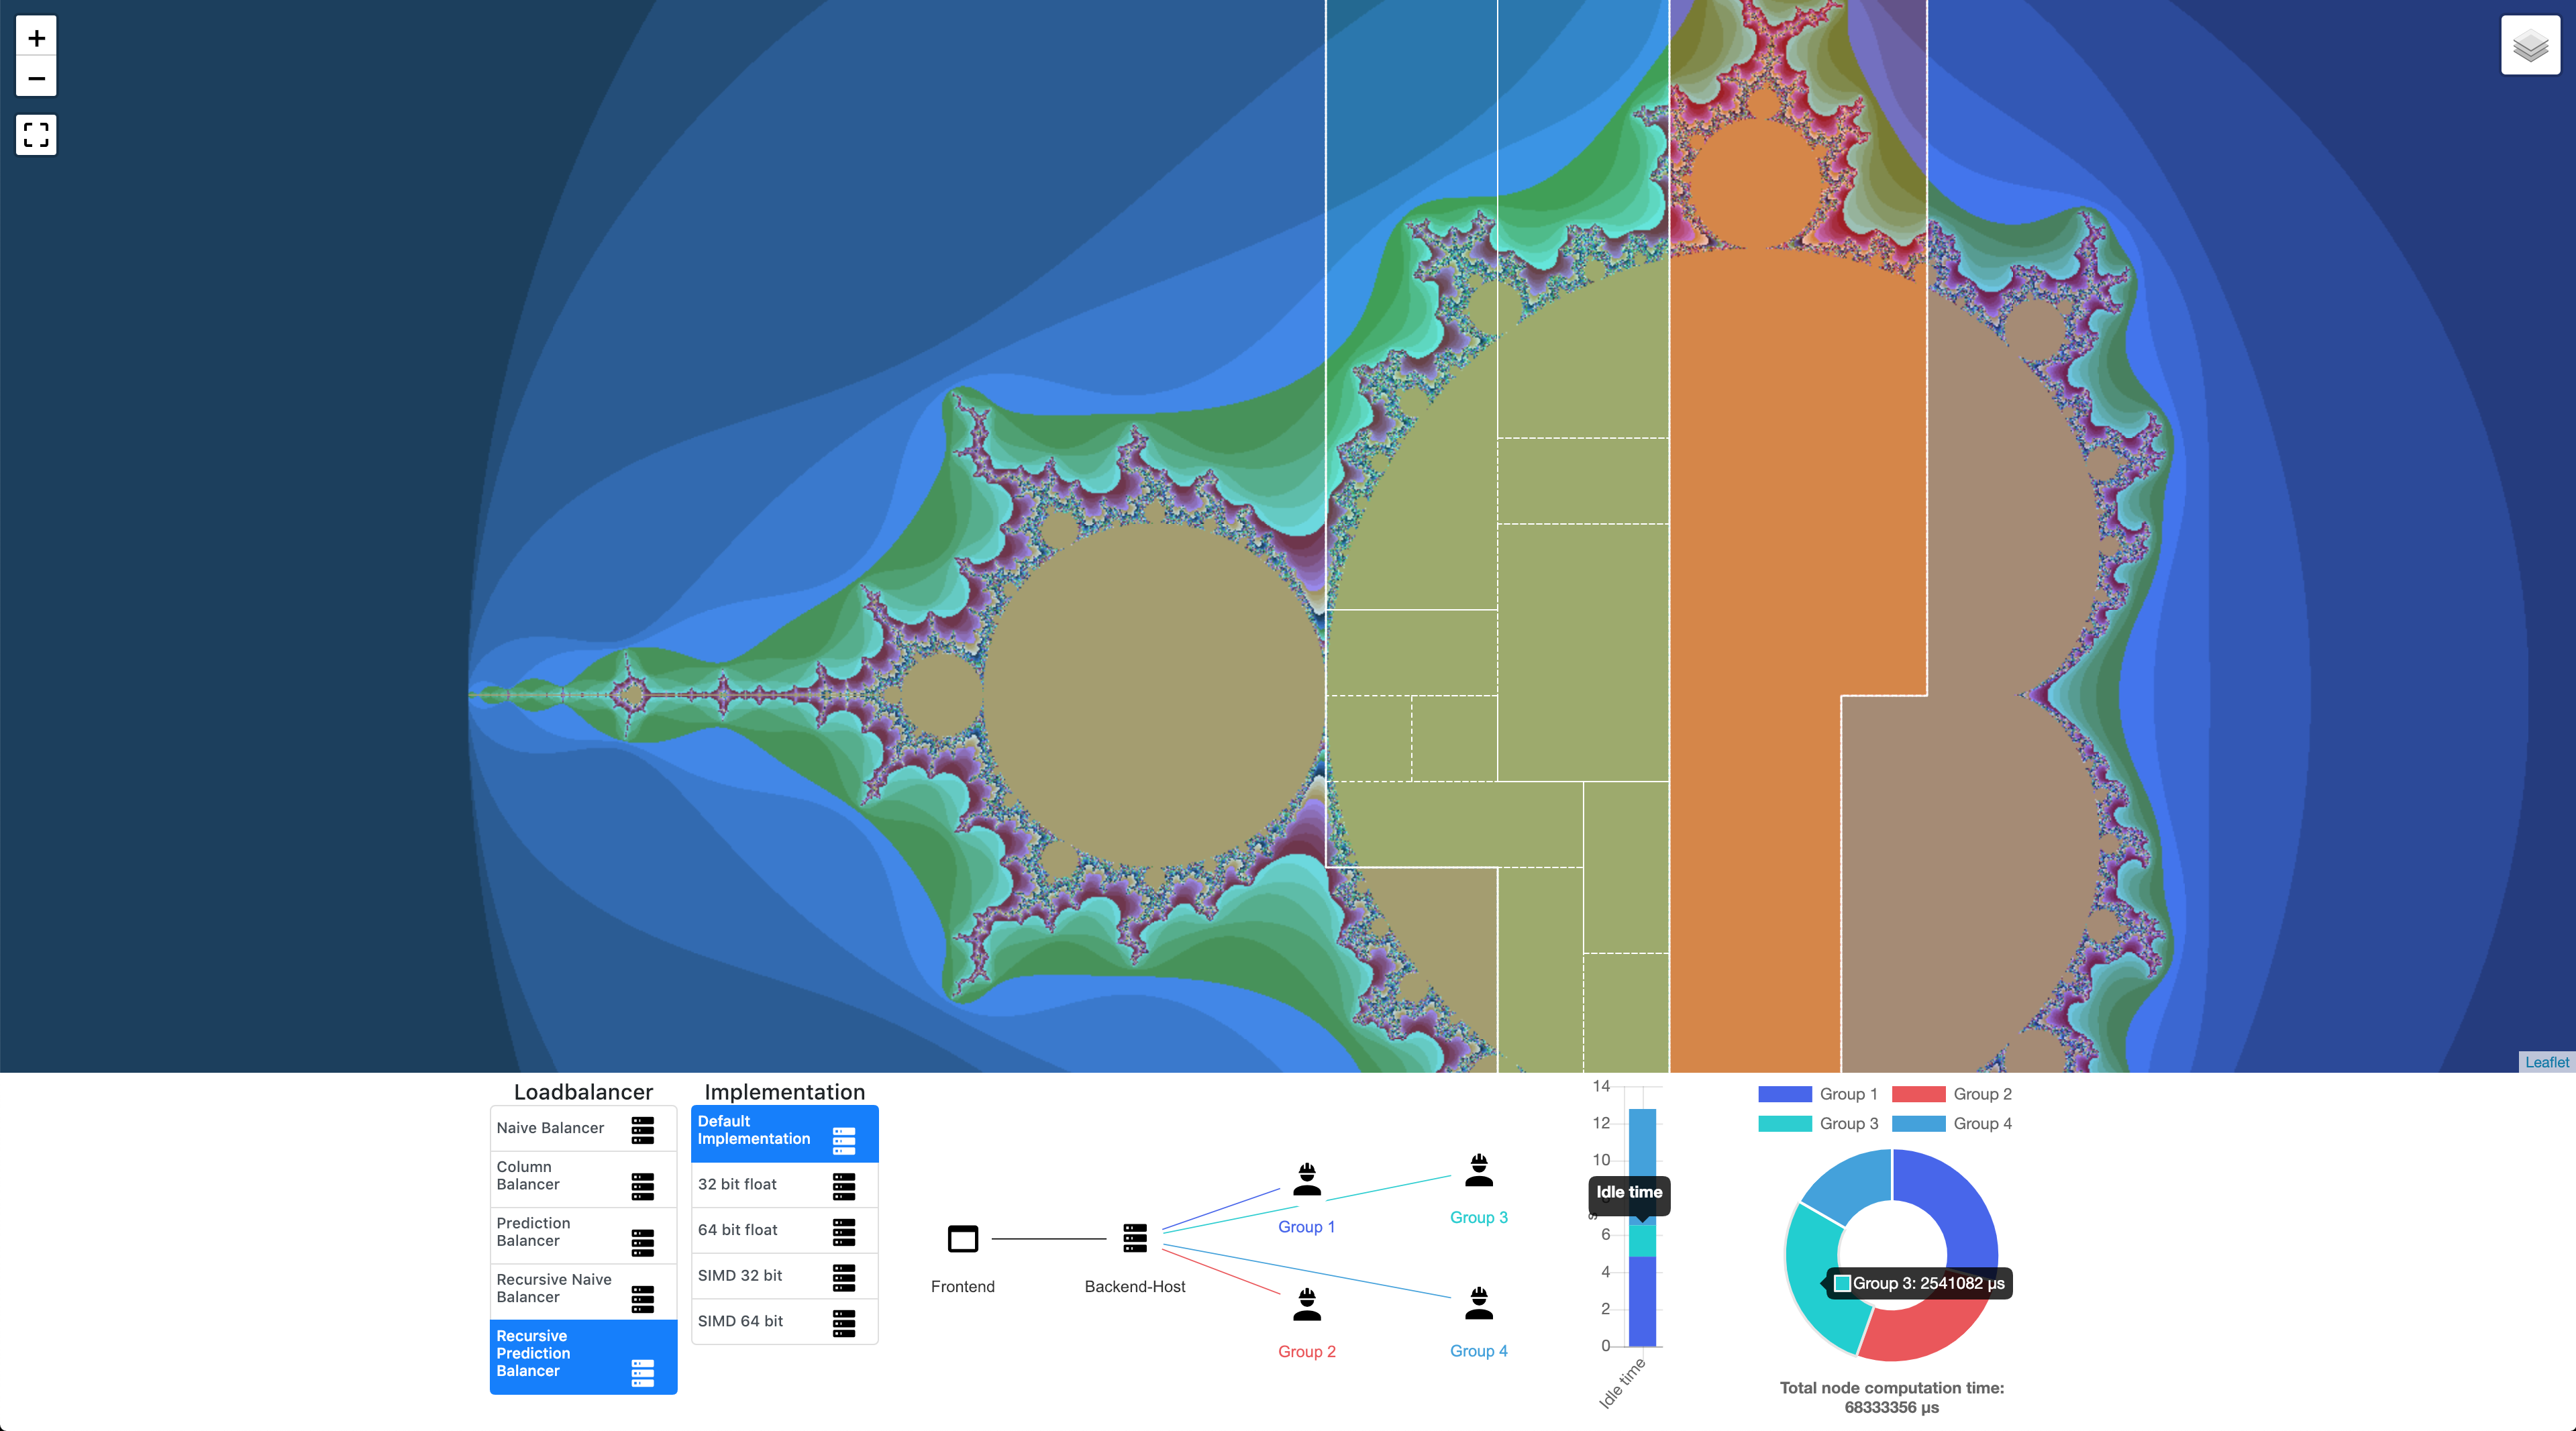
\includegraphics[width=\linewidth]{img/Implementierung/UI-Screenshot}
	\caption{Benutzeroberfläche der Mandelbrot Anwendung}
	\label{fig:ui-screenshot}
\end{figure}

Um das Frontend zu implementieren, wurde sich für die Programmiersprache TypeScript\footnote{\url{https://www.typescriptlang.org/}}(Erweiterung von JavaScript um Typisierung) entschieden.
Da diese zu JavaScript kompiliert, werden die Vortele von JavaScript, wie Ausführung im Webbrowser des Benutzers und eine vielzahl verfügbarer Bibliotheken,
mit den Vorteilen einer typisierten Programmiersprache vereint.

Für die graphische Benutzeroberfläche wurde ebenfalls TypeScript mit dem React Framework\footnote{\url{https://reactjs.org/}} verwendet, welches es ermöglicht,
graphische Komponenten nativ in TypeScript zu erstellen und verändern.
Es wurde für jede Komponente eine eigene TypeScript Klasse zu erstellt, welche dann den betreffenden
das betreffende Verhalten und dessen Darstellung enthält.

Um das Fraktal darzustellen wird die Leaflet\footnote{\url{https://leafletjs.com/}} Bibliothek verwendet.
Diese, für Onlinekarten konzipierte, Bibliothek stellt den Bereich der komplexen Ebene, auf der die Mandelbrotmenge liegt dar.
Dabei wird der momentan sichtbare Ausschnitt der Menge mit Hilfe der WebSockets Verbindung (siehe \autoref{sec:fontend_communication}) an das Backend versendet und vom ausgewählten Lastbalancierer in Teilregionen unterteilt (siehe \autoref{sec:load_balancing}).
Jeder der vom Backend berechneten Teilregionen wird, sobald diese empfangen wurden, im Frontend angezeigt und die Komponenten
zu Visualisierung der Rechenzeit aktualisiert.

\subsubsection{Kommunikation mit dem Backend}\label{sec:fontend_communication}

Zur Kommunikation mit dem Backend wird im Frontend ein Objekt der Klasse \texttt{WebSocketClient} erzeugt.
Die zur Verbindung verwendeten Codestücke liegen dabei alle in dem Ordner \verb|connection|, die genannte Klasse wird in
\verb|WSClient.ts| definiert.

Die dort definierte Klasse \verb|WebSocketClient| abstrahiert von dem JavaScript-nativen Websocketinterface \verb|WebSocket|\footnote{\url{https://developer.mozilla.org/en-US/docs/Web/API/WebSocket}}.
Bei der Initialisierung baut das erzeugte Objekt eine Verbindung zu der lokalen Adresse \url{ws://localhost:9002} auf\footnote{
	Faktisch wird eine Verbindung geöffnet, geschlossen und erneut geöffnet.
	Dies ist durch ein ungelöstes Problem beim Verbindungsaufbau bedingt, das dafür sorgt, dass ein Verbindungsaufbau
	erst bei der zweiten erzeugten Websocketverbindung fehlerfrei gelingt.
}.
Dort sollte das Backend bereit sein, eine Websocketverbindung anzunehmen.

Zudem bietet die Klasse die Methode \texttt{sendRequest}, welche ein übergebenes RegionRequest-Objekt JSON-kodiert und versendet.

Wichtig für den Rest des Frontends sind die Methoden \texttt{registerRegion} und \texttt{registerRegionData}.
An diese Methoden können Callbacks übergeben werden, die aufgerufen werden, wenn das Frontend über die Websocketverbindung
respektive ein \texttt{Region}-Objekt oder ein \texttt{RegionData}-Objekt empfängt.
Diese sind die Aufteilung einer angefragten Region (siehe \autoref{src:region.json})
oder die berechneten Iterationswerte einer Region (siehe \autoref{src:regionData.json}).
Die übergebenen Callbacks erhalten als Parameter respektive die vorgruppierte Aufteilung als ein Array von Workergruppen (\texttt{RegionGroup})
oder das JSON-dekodierte \verb|RegionData|-Objekt.

Zudem wird hierbei bereits eine Filterung der eingehenden Regionsdaten vorgenommen.
Bei Empfang einer Regionsaufteilung, wird diese zwischengespeichert.
Jedes empfangene Regionsdatenobjekt wird dann bei Empfang daraufhin überprüft,
ob der darin dargestellte Ausschnitt einer Regionsaufteilung entspricht (dazu wird das \verb|region|-Attribut verglichen)
und das dargestellte Fraktal der zuletzt übergebenen Auswahl entspricht.
Diese Filtrierung ist notwendig, da Worker Regionsdaten auch "verspätet" absenden können,
falls bei dem zuvorgehenden Bereich nicht gewartet wurde bis die Berechnungen aller Worker entgegengenommen wurden.

Die Definitionen der zugehörigen Objekt-Interfaces finden sich in den Dateien \verb|RegionGroup.ts| und \verb|ExchangeTypes.ts|.

Als weitere Hilfsfunktion wird in \verb|RegionRequest.ts| \verb|request| bereitgestellt.
Diese extrahiert aus der übergebenen Sicht auf die Mandelbrotmenge, die in der Leaflet-Karte gespeichert ist,
die Parameter zum Anfragen einer Region.
Dazu werden mithilfe des aktuellen Zooms der linke obere und rechte untere Punkt des Sichtbereiches
in dem Leaflet-internen Koordinatensystem auf entsprechende Punkte in der komplexen Ebene projeziert.
Da zum Erzeugen des passenden Objektes auch der gewünschte Lastbalancierer und der Fraktaltyp notwendig sind,
werden diese als weitere Parameter übergeben.
Die Funktion gibt direkt ein Objekt zurück, dass das Interface \verb|RegionRequest| erfüllt.

\subsubsection{Darstellung der Regionsdaten} % tileDisplay/

Die für die Darstellung der Mandelbrotmenge verwendete Bibliothek (leaflet) hat die Einschränkung, dass
nur Quadrate einer vordefinierten Größe (\verb|Tiles|) angezeigt werden können. Ebenfalls verwendet diese ein
eigenes Koordinatensystem, unter welchem jede angezeigte Tile eindeutig mit dem Tripel \( (x, y, zoom) \)
identifiziert wird. Somit ist eine Übersetzung zwischen den Daten des Backends und den von leaflet erwarteten nötig.

\paragraph{MatrixView.ts, RegionOfInterest.ts}\label{par:matrixView}
Die Klasse \verb|MatrixView.ts| implementiert die Umsetzung einer vom Backend versendeten Region zu
den von leaflet erwarteten Tiles. Dafür registrieren sich alle sichtbaren Tiles durch die Methode
\verb|registerTile(point, draw)| mit dem Callback \verb|draw|, welcher ausgeführt wird, sobald die anzuzeigenden Daten für die
entsprechende Tile verfügbar sind. Diese Iterationswerte des Backends werden dabei der \verb|draw| Funktion als Parameter
in Form eines \verb|RegionOfInterest| Objekts übergeben.

Ein \verb|RegionOfInterest| Objekt implementiert wiederum die Übersetzung von lokalen \( (x,y) \) Pixel-Werten
einer Tile zu Indizes in die vom Backend gesendeten Regionsdaten (siehe \autoref{src:regionData.json}). Dabei gibt die
\verb|get(x, y)| Methode, für einen Tile \( (x,y) \) Pixel-Wert die benötigte Iterationsanzahl zurück (siehe \autoref{src:RegionOfInterest.ts}).

\begin{figure}[h!]
	\lstinputlisting[caption={Umsetzung von Pixel-Werten der Tiles zu Indizes in Regionsdaten}, label={src:RegionOfInterest.ts}, language=TypeScript, firstline=39, lastline=46, firstnumber=39]{../../frontend/src/tileDisplay/RegionOfInterest.ts}
\end{figure}

\paragraph{TileDisplay.tsx}
Die Klasse \verb|TileDisplay.tsx| verwendet die leaflet Bibliothek direkt, um die Regionsdaten darzustellen.
Dabei wird dieser die WebSocket Verbindung in Form eines \verb|WebSocketClient|, sowie der vom Nutzer gewählte Balancer,
die Implementierung und Gruppierung durch \verb|Observable| Klassen (siehe \autoref{par:observables}) übergeben. Ebenfalls wird der anzuzeigende Ausschnitt der
Mandelbrotmenge übergeben.

\begin{figure}[h!]
	\centering
	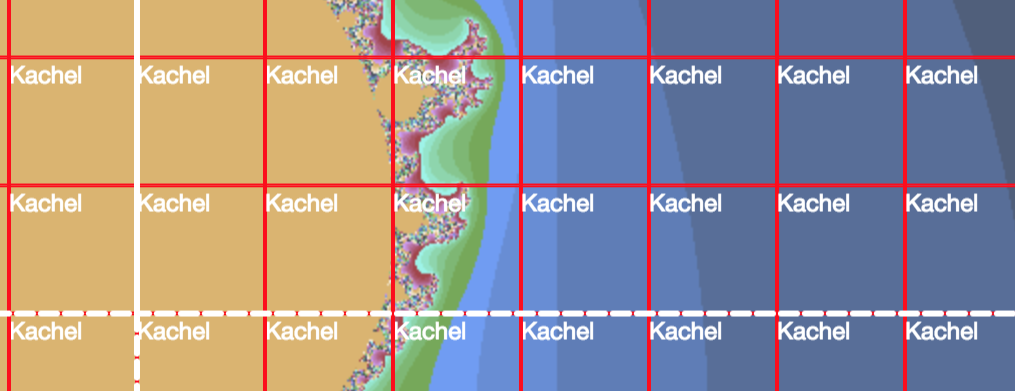
\includegraphics[width=0.5\linewidth]{img/Implementierung/leafletTiles}
	\caption{Relation von Backend Regionen zu leaflet Tiles}
	\label{fig:leafletTiles}
\end{figure}

Da das Backend die berechneten Teilbereiche der Mandelbrotmenge als Regionen zurück gibt, dessen Höhe und Breite
Vielfache der leaflet Tile-Größe sind, wird eine Region dem Benutzer durch mehrere Tiles dargestellt.
Dieses Verhältnis wird in \autoref{fig:leafletTiles} dargestellt. Dabei ist beispielhaft eine Region des Backends
weiß eingezeichnet, alle leaflet Tiles sind rot umrandet angegeben. Eine detailliertere Version dieser Anzeige kann
durch die Auswahl des \verb|DebugLayer|s jederzeit im Frontend eingeblendet werden.

Dargestellt werden die Tiles in einer eigenen Ebene der leaflet Karte, dem \verb|MandelbrotLayer|.
Dieser erstellt für den sichtbaren Bereich\footnote{Da die Fenstergröße des sichtbaren Bereichs keien Vielfaches der Tilegröße sein muss, können Tiles erzeugt werden, welche teilweise außerhalb des sichtbaren Beriechs liegen}
alle benötigten Tiles. Für jede der Tiles wird ein \verb|HTML5 canvas|\footnote{\url{https://developer.mozilla.org/kab/docs/Web/API/Canvas_API}} Objekt erstellt, welches es
ermöglicht, für jeden Pixel einen \( (r,g,b) \) Farbwert zu definierten und anzuzeigen. Wobei die Farbwerte aus den berechneten
Iterationswerten des Backends mit einem Shader (siehe \autoref{par:shader}) ermittelt werden. Die Iterationswerte können wiederum
mit einem \verb|MatrixView| Objekt aus den Regionsdaten des Backends gelesen werden.

Weiterhin wird in \verb|TileDisplay| der \verb|WorkerLayer| (siehe \autoref{par:workerLayer}), welcher die Regionsaufteilung des Backends visualisiert,  hinzugefügt und callbacks auf die Observables definiert, welche die momentan sichtbare Region
erneut vom Backend anfordern, falls sich einer der ausgewählten Lastbalancierer, oder die gewählte Implementierung ändert.

\paragraph{Shader.ts}\label{par:shader}
Berechnet für einen Iterationswert der Mandelbrotmenge ein Tripel \( (r,g,b) \) von Farbwerten.
Implementiert ist eine simple Funktion, welche den Iterationswert für jeden Farbkanal mit einer Konstante multipliziert
und auf den zulässigen ganzzahligen Wertebereich \( [0,255] \) abbildet (siehe \autoref{src:Shader.ts}).

\begin{figure}[h!]
	\lstinputlisting[caption={Berechnung der \( (r,g,b) \) Farbwerte}, label={src:Shader.ts}, language=TypeScript, firstline=2, lastline=7, firstnumber=2]{../../frontend/src/tileDisplay/Shader.ts}
\end{figure}

\paragraph{Project.ts}
Da die leaflet Bibliothek Tiles verwendet, um die Regionen des Backends anzuzeigen, liegen diese Tiles in 
einem neuen Koordinatensystem, welches jeder Tile auf einer Zoomstufe ein Triple \( (tileX, tileY, zoom) \)
zuordnet. Weiterhin besitzt leaflet ein internes Koordinatensystem (CRS\footnote{\url{https://en.wikipedia.org/wiki/Spatial_reference_system}}),
welches jeden Punkt auf der Karte durch das Paar \( (latitude, longitude) \) identifiziert. 
\verb|Projekt.ts| enthält Funktionen, um zwischen diesen 3 Koordinatensystemen (Tile-Koordinaten, leaflet-Koordinaten 
und Koordinaten der komplexen Ebene) zu konvertieren.

\paragraph{Regionsgruppierung (RegionGroup.ts)}\label{par:regionGroup}

\paragraph{WorkerLayer.ts}\label{par:workerLayer}
Diese Klasse visualisiert die Regionsaufteilung des Lastbalancierers als Overlay, welche über den Iterationswerten
dem Benutzer angezeigt wird. Dafür wir eine in leaflet bestehende \verb|GeoJSON| API verwendet, mit welcher es möglich
ist, beliebige Polygone auf den bestehenden Kartendaten anzuzeigen. Die Eckpunkte für diese Polygone für jede \verb|RegionGroup| 
mit Hilfe der Funktionen aus \verb|Project| von Koordinaten der komplexen Ebene, welche im Backend verwendet werden, zu 
leaflet Koordinaten umgerechnet.

\begin{figure}[h!]
	\centering
	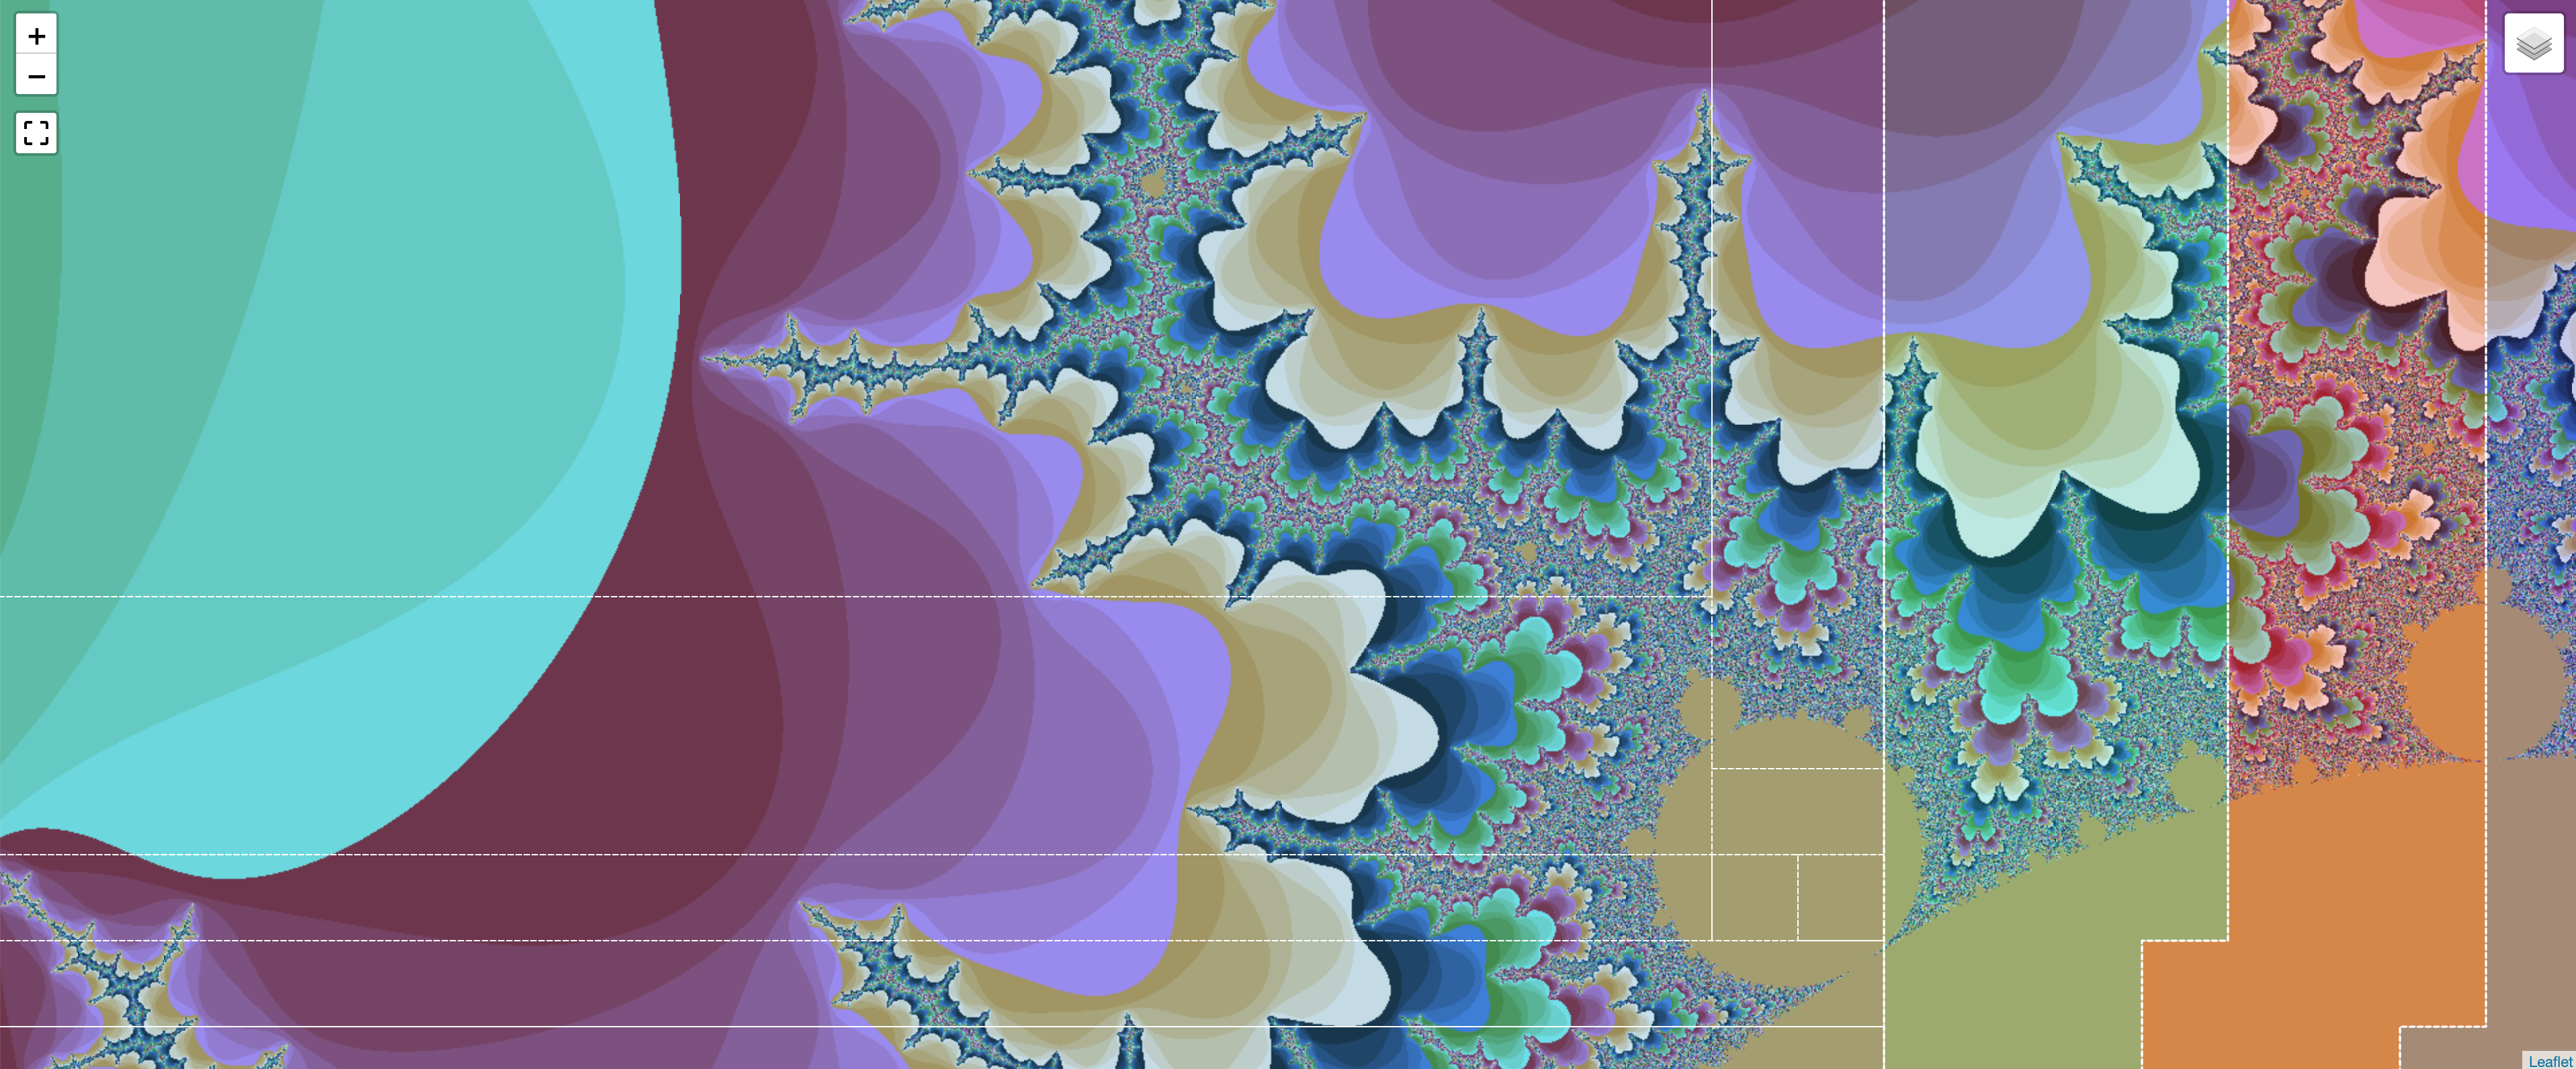
\includegraphics[width=\linewidth]{img/Implementierung/regionGrouping}
	\caption{Gruppierung einer Aufteilung des Recursive PredictionBalancers mit 37 Workern}
	\label{fig:regionGrouping}
\end{figure}

Da es wie in \autoref{par:regionGroup} beschrieben zu einer Gruppierung kommt, falls die Anzahl der Worker im Backend zu
groß ist, werden ebenfalls alle Untergruppen einer Gruppe angezeigt (siehe \autoref{fig:regionGrouping}), falls der Benutzer mit der Maus über eine der 
dargestellen Gruppierungen geht.

\subsubsection{Visualisierung der Programmstruktur}

Die Struktur der Parallelisierung wird in einem Netzwerkgraphen unter dem Fraktal dargestellt.
Mithilfe der Bibliothek \verb|visjs|\footnote{\url{http://visjs.org/}} wird hierzu ein
Graph mit 3 Ebenen erzeugt: Auf der linken Seite befindet sich ein Knoten in Form eines Programmfensters, der das Browserfrontend darstellt.
In der Mitte wird ein Knoten für den Backend-Host mit Serverrack als Symbol dargestellt, der mit dem Frontendknoten verbunden ist.
Auf der rechten Seite befindet sich schließlich zwischen 2 und 4 Knoten, die jeweils eine Gruppe an Arbeitern
darstellen. Das Symbol hierfür ist ein Oberkörper mit Arbeitshelm.
Sie sind wiederum direkt mit dem Host verbunden.

Der Code für diese Darstellung findet sich in \verb|components/NetworkView.tsx|.
Dort wird ein Baumgraph von links nach rechts mit manueller Ebenenverteilung als Grundstruktur für die Darstellung des Graphen definiert.
Daher wird das Frontend auf der höchsten Ebene und der Backend-Host auf der Ebene darunter spezifiziert.
Die Arbeiter werden auf Basis der erhaltenen Regionsaufteilung erzeugt und jeweils zu zweit nacheinander
auf Ebenen verteilt.
Diese Aufteilung wird nach Erhalt jeder Regionsaufteilung vorgenommen und der Graph neu aufgebaut,
sowie die Größe der Leinwand an die Anzahl an Knoten angepasst.

\subsubsection{Visualisierung der Rechenzeiten} % components/

Die zeitbezüglichen Komponenten der Visualisierung werden mithilfe der Charts
der Bibliothek \verb|chartjs|\footnote{\url{http://www.chartjs.org/}} dargestellt.

\paragraph{Idle Time}

Für die kritische Information der verschwendeten Zeit wird ein Balkengraph verwendet.
Dieser besitzt einen Balken, der die Differenz zwischen der Rechenzeit aller Knoten und dem am längsten rechnenden Knoten
aufsummiert und nach Gruppe sortiert darstellt.
Die Darstellung wird bei Empfang einer Regionsaufteilung (mithilfe \verb|registerRegion| in dem Websocketclient)
initialisiert indem die Anzahl an Knoten und die Gruppen gespeichert, die Rechenzeit der Knoten auf 0 gesetzt und 
alle Knoten als aktiv markiert werden.
Da die tatsächliche Rechenzeit erst am Ende der Berechnung mit den Regionsdaten selbst verfügbar ist,
wird mithilfe eines Intervalls die Rechenzeit live abgeschätzt, indem sie simpel alle 50 Millisekunden
um 50 Millisekunden hochgezählt wird, falls die Regionsdaten des Knotens noch nicht empfangen wurden.
Da die Charts nicht zur Animation von Übergängen fähig sind, wird das Objekt mit jedem Update neu gerendert.
Bei Empfang von Regionsdaten (hierzu wird die erwähnte Methode \verb|registerRegionData| verwendet) 
wird die tatsächlich gemessene Rechenzeit eingetragen und der Rechenknoten als inaktiv gekennzeichnet.
Der Intervall wird gestoppt, sobald alle Arbeiterknoten die Berechnung abgeschlossen haben.
Einiges an Code ist dabei nur dafür zuständig, beim Schweben über einem Teil des Balkens die Wartezeit
einer einzelnen Gruppe in einem Tooltip darzustellen.

\paragraph{ComputationTime}

Zur Darstellung des relativen Verhältnisses der Rechenzeiten wird in einem Kuchengraph
die absolute Rechenzeit der Gruppen dargestellt.

\subsubsection{MISC} % misc/

\paragraph{Observable.ts}\label{par:observables}